\documentclass[handout,usenames,dvipsnames]{beamer} % To enable \pause: remove the "handout" preamble
\usetheme{Boadilla}
\usecolortheme{default}
\usepackage{pgfpages}
% \setbeameroption{hide notes} % Only slides
% \setbeameroption{show only notes} % Only notes
\setbeameroption{show notes on second screen=right} % Both
\setbeamertemplate{note page}{\pagecolor{yellow!5}\insertnote}\usepackage{palatino}

\usepackage[utf8]{inputenc}
\usepackage[round]{natbib}
\renewcommand*{\bibfont}{\scriptsize}
\usepackage{tikz}
\usepackage{wrapfig}

\DeclareMathOperator{\rank}{rank}
\DeclareMathOperator{\erank}{erank}
\DeclareMathOperator{\cl}{cl}
\DeclareMathOperator{\diag}{diag}
\DeclareMathOperator{\spn}{span}
% \newtheorem{theorem}{Theorem}
\newtheorem{assumption}{Assumption}
% \newtheorem{definition}{Definition}
\newtheorem{observation}{Observation}
% \newtheorem{corollary}{Corollary}
% \newtheorem{lemma}{Lemma}
\usepackage{dsfont}
\newcommand{\onefunc}{\mathds{1}}
\newcommand{\din}{{d_{\text{in}}}}
\newcommand{\dhid}{{d_{\text{hidden}}}}
\newcommand{\dout}{{d_{\text{out}}}}
\newcommand{\eps}{\epsilon}
\newcommand{\TODO}{\Red{TODO}}
\newcommand{\abs}[1]{\left|{#1}\right|}
\newcommand{\tr}[1]{\text{Tr}\left({#1}\right)}
\newcommand{\vect}[1]{\text{vec}\left({#1}\right)}
\newcommand{\opt}[1]{#1^\star}
\newcommand{\norm}[2][]{{\left\|{#2}\right\|_{#1}}}
%\newcommand{\norm}[1]{\left\|#1\right\|}
\newcommand{\snorm}[1]{\|#1\|} %small norm
\renewcommand{\angle}[2]{\measuredangle \left( #1, #2 \right)}
\newcommand{\bigangle}[2]{\measuredangle \left\big( #1, #2 \right\big)}
\newcommand{\Red}[1]{\colorbox{red}{#1}}
\newcommand{\set}[1]{\left\{{#1}\right\}}

\newcommand{\ba}{\mathbf{a}}
\newcommand{\be}{\mathbf{e}}
\newcommand{\bx}{\mathbf{x}}
\newcommand{\bw}{\mathbf{w}}
\newcommand{\bg}{\mathbf{g}}
\newcommand{\bb}{\mathbf{b}}
\newcommand{\bu}{\mathbf{u}}
\newcommand{\bv}{\mathbf{v}}
\newcommand{\bz}{\mathbf{z}}
\newcommand{\bc}{\mathbf{c}}
\newcommand{\br}{\mathbf{r}}
\newcommand{\bd}{\mathbf{d}}
\newcommand{\bp}{\mathbf{p}}
\newcommand{\bh}{\mathbf{h}}
\newcommand{\by}{\mathbf{y}}
\newcommand{\bn}{\mathbf{n}}
\newcommand{\bs}{\mathbf{s}}
\newcommand{\bq}{\mathbf{q}}
\newcommand{\bmu}{\boldsymbol{\mu}}
\newcommand{\balpha}{\boldsymbol{\alpha}}
\newcommand{\bbeta}{\boldsymbol{\beta}}
\newcommand{\btau}{\boldsymbol{\tau}}
\newcommand{\bxi}{\boldsymbol{\xi}}
\newcommand{\blambda}{\boldsymbol{\lambda}}
\newcommand{\bepsilon}{\boldsymbol{\epsilon}}
\newcommand{\bsigma}{\boldsymbol{\sigma}}
\newcommand{\btheta}{{\boldsymbol{\theta}}}
\newcommand{\bomega}{\boldsymbol{\omega}}
\newcommand{\Xcal}{\mathcal{X}}

\newcommand{\co}{{\cal O}}
\newcommand{\ca}{{\cal A}}
\newcommand{\cb}{{\cal B}}
\newcommand{\cd}{{\cal D}}
\newcommand{\cdb}{{\cal D}^{\rm b}}
\newcommand{\cc}{{\cal C}}
\newcommand{\ck}{{\cal K}}
\newcommand{\cq}{{\cal Q}}
\newcommand{\ce}{{\cal E}}
\newcommand{\ct}{{\cal T}}
\newcommand{\cg}{{\cal G}}
\newcommand{\ch}{{\cal H}}
\newcommand{\cm}{{\cal M}}
\newcommand{\ci}{{\cal I}}
\newcommand{\cj}{{\cal J}}
\newcommand{\cw}{{\cal W}}
%\newcommand{\cl}{{\cal L}}
\newcommand{\cf}{{\cal F}}
\newcommand{\cv}{{\cal V}}
\newcommand{\cp}{{\cal P}}
\newcommand{\cu}{{\cal U}}
\newcommand{\cx}{{\cal X}}
\newcommand{\cy}{{\cal Y}}
\newcommand{\cz}{{\cal Z}}
\newcommand{\cs}{{\cal S}}
\newcommand{\cn}{{\cal N}}
\newcommand{\calr}{{\cal R}}

\newcommand{\bbs}{{\mathbb S}}
\newcommand{\reals}{{\mathbb R}}
\newcommand{\nat}{{\mathbb N}}
\newcommand{\integers}{{\mathbb Z}}
\newcommand{\complex}{{\mathbb C}}
\newcommand{\zero}{{\mathbf{0}}}

% Style conventions
\newcommand{\true}[1]{{\textcolor{ForestGreen}{\textbf{#1}}}}




\title[Implicit Reg.: Rank Min. in ReLU Networks]{Implicit Regularization Towards Rank Minimization in ReLU Networks}
\author[Nadav Timor]{
    by Nadav Timor\newline
    Advisor: Prof. Ohad Shamir
}
\institute[Weizmann Institute]{Weizmann Institute of Science}
\date[March 2022]{
    March 2022 \newline \newline \newline \newline \newline
    {
        \footnotesize
        Based on a joint paper with Gal Vardi and Ohad Shamir (under review in ICML'22).
    }
}
% \logo{
\includegraphics[height=.75cm]{WeizmannLogo.png}}



\begin{document}



\frame{\titlepage}




\section{Preliminaries}

\begin{frame}{Table of Contents}
    \tableofcontents[currentsection]
    
    \note{
        We have results for both the square~loss and classification~losses that I split into two different~sections. I thought to~start with a high-level~view of our~work where we skip some~slides that we could cover later. Then, we dive into results and their proof~ideas, at~your~preference.
    }
\end{frame}



\begin{frame}{Preliminaries}
    \pause
    \begin{definition}[fully-connected~neural~network]
        A fully-connected~neural~network $N_\btheta$ of depth~$k \geq 2$ is parameterized by a collection~$\btheta := [W^{(\ell)}]_{\ell=1}^k$ of weight~matrices\\
        ($\forall \ell \in [k] : W^{(\ell)} \in \reals^{d_\ell \times d_{\ell-1}}$), and computes a function $N_\btheta : \reals^\din \to \reals^\dout$:
        \[
            N_\btheta(\bx) := 
            \onslide<5->{W^{(k)}}
                \onslide<4->{\sigma\Big( W^{(k-1)} \ldots }
                    \onslide<3->{\sigma\Big( W^{(2)}~} 
                        \sigma\Big( W^{(1)} \bx \Big) 
                    \onslide<3->{\Big)}
                \onslide<4->{ \Big)} 
            \onslide<5->{\Big)}
            , \forall \bx
        \]
        where $\sigma:\reals \to \reals$ is an activation~function that acts coordinate-wise.
    \end{definition}
    \onslide<6->{
        \begin{description}
            \item[fully-connected \emph{linear} neural~network] $N_\btheta$, where $\sigma$ is the identity.
            \item[fully-connected \emph{ReLU} neural~network] $N_\btheta$, where $\sigma(z) := \max\set{0, z}$.
        \end{description}
    }
    \onslide<7->{
        \begin{description}
            \item[overparameterized neural network] $N_\btheta$, where $\prod_{\ell = 1}^k d_\ell \cdot d_{\ell-1} >> n \cdot \din$.
        \end{description}
    }
    
    \note{
        \scriptsize
        \begin{enumerate}
            \itemsep=0pt
            \topsep=0pt
            \item We concern a fully-connected~neural~network, denoted by $N_\btheta$, where $\btheta$ is a collection of $k$ weight~matrices $W^{(\ell)}$. We say that $k$ is the \emph{depth} of the network, and it is $\ge 2$. The network computes a function $\reals^{\din} \to \reals^{\dout}$ in the following iterative way. A given input vector $\bx$ is multiplied by the first weight matrix, $W^{(1)}$. On the resulted multiplication, we apply an entrywise real-valued function, denoted by $\sigma$. This expression is called ``the output of the first layer" or ``the input to the second layer".
            \item Then, we repeat: We take the output of the first layer and do the same: Multiplying by $W^{(2)}$ and applying $\sigma$.
            \item This continues until we compute the input to the last layer.\\
            \item Then, we only multiply by the last weight matrix, $W^{(K)}$. Note that we do not have an activation function in the last layer or bias terms.\\
            The $d_\ell$ rows of $W^{(\ell)}$ are ``the neurons of the $\ell$-th layer". The \emph{hidden neurons} are the neurons in all layers except the last (namely, in layers $1, \ldots, k-1$). The \emph{width of the $\ell$-th layer} is the number of its neurons, and the \emph{width of the network} is the maximal width of all layers.
            \item When referring to a \emph{linear} network, we mean that $\sigma$ is the identity function. \emph{ReLU} network is when $\sigma$ is the $\max$ between $0$ and its input.
            \item An \emph{overparameterized}~network~$N_\btheta$ has far more learnable~parameters than training~examples.
        \end{enumerate}
    }
\end{frame}



\begin{frame}
    \pause
    \begin{definition}[square loss]
        
        Given a network $N_\btheta$ and a dataset $\{(\bx_i,\by_i)\}_{i=1}^n \subseteq \reals^\din \times \reals^\dout$,
        \begin{align*} \label{eq:objective}
        	 L_{X,Y}(\btheta) 
        	 := \frac{1}{2} \sum_{i=1}^n \norm{N_\btheta(\bx_i) - \by_i}^2
        	 = \frac{1}{2} \norm{N_\btheta(X) - Y}_F^2~.
        \end{align*}
        $(X,Y) \in \reals^{\din \times n} \times \reals^{\dout \times n}$ are the corresponding data matrices.
    \end{definition}
    \pause
    \begin{itemize}
            \item Assume $\min_\btheta L(\btheta)=0$.
            \pause
            \item Overparameterization $\Rightarrow$ Multiple (or even $\infty$) global minima.
        \end{itemize}
    \pause
    \begin{definition}[gradient flow (w.r.t. square loss)]
        Let~$\btheta(t)$ be the trajectory of GF. Starting from $\btheta(0)$, the dynamics is given by $\frac{d \btheta(t)}{dt} = -\nabla L_{X,Y}(\btheta(t))$.
    \end{definition}
    \begin{itemize}
        \pause
        \item GF \emph{converges} $\Leftrightarrow \btheta(\infty) := \lim_{t \to \infty}\btheta(t)$.
        % \pause
        % \item Assume $\sigma'(0) = 0$ for convenience.
    \end{itemize}
    
    \note{
        \footnotesize
        \begin{enumerate}
            \item The \emph{empirical square loss} is half the sum of the squared~$\ell_2$-norm of the differences between the network’s prediction,~$N_\btheta(\bx_i)$, and the corresponding target~vector,~$\by_i$. For~convenience, we sometimes use the matrix~notation and take the Frobenius~norm. Then, we stack the input~and~target~vectors as the columns of the matrices~$X, Y$.
            \item In all our results, we assume that the data is \emph{realizable}. Namely, there exists a parameterization $\btheta$ attaining $0$~loss.
            \item We also assume to have overparameterized~networks so~that $L$ has multiple (or even infinitely~many) global~minima.
            \item We consider GF with the square~loss. It captures the behavior of GD with an infinitesimally~small~step~size. $\btheta(t)$ is the trajectory of GF, starting from an initial~point~$\btheta(0)$. The following differential~equation gives the dynamics of~$\btheta(t)$: The derivative~of~$\btheta(t)$ equals minus~the~gradient of the objective~function~$L_{X,Y}$ with~respect~to~$\btheta(t)$.
            \item We say that GF~\emph{converges} if $\lim_{t \to \infty}\btheta(t)$~exists, and we denote this limit by $\btheta(\infty)$.\\
            Note that we assume that the derivative~of~the~ReLU at~$\zero$ equals~$0$.
            % \item Another note is that, by default, the derivative of the ReLU~function at $\zero$ is ambiguous. However, practical implementations of gradient~methods define its derivative~at~$\zero$ to be some constant in the closed~interval between $0$~and~$1$ ((N.T.:~$\sigma'(0) \in [0,1]$)). For convenience, we assume that the derivative~at~$\zero$ equals~$0$.
        \end{enumerate}
    }
\end{frame}





\begin{frame}{What is \emph{implicit regularization}?}{Generalization despite overparameterization}
    \pause
    Setting: \#[learnable parameters] $>>$ \#[training examples].
    \pause
    \begin{itemize}
        \item $\Rightarrow$ \alert{Many} global minima with $0$ training loss.
    \end{itemize}
    \pause
    \begin{block}{Phenomenon in practice (\cite{zhang2017understanding})}
        GD over overparameterized neural networks prefers solutions that generalize well even when trained \true{without~explicit~regularization}.
    \end{block}
    \textbf{Q:} How?\\
    \pause
    \textbf{Possible A:} \emph{``implicit regularization''} (or \emph{``implicit bias''}).
    
    \note{
        \footnotesize
        \begin{enumerate}
            \item As said, we focus on overparameterized~networks, namely, models with far more learnable~parameters than training~examples.
            \item In this setting of learning, we face an underdetermined optimization~problem with many global~minima of $0$~training~loss.
            \item A central puzzle in the theory~of~deep~learning is how such overparameterized neural~networks generalize, even when trained without explicit~regularization, as \cite{zhang2017understanding}  demonstrated.
            \item A possible explanation is that GD induces an {\em implicit~regularization}~(or~\emph{implicit~bias}).
        \end{enumerate}
        Today we take another step in trying to characterizing this regularization/bias.
        
        \vspace*{\fill}
        \noindent\rule{\textwidth}{1pt}
        \newline
        \alert{If asked:}
        \begin{itemize}
            \item \cite{zhang2017understanding}: Large CNNs,\\
            trained with stochastic~gradient~methods\\
            fit a random~labeling (of the training~data), or even completely~unstructured random~noise.\\
            Unaffected by explicit~regularization.
        \end{itemize}
    }
\end{frame}




\begin{frame}{What is \emph{implicit regularization/bias}?}
    \tikzset{every picture/.style={line width=0.75pt}} %set default line width to 0.75pt        
    
    \begin{tikzpicture}[x=0.75pt,y=0.75pt,yscale=-1,xscale=1]
        % uncomment if require: \path (0,261); %set diagram left start at 0, and has height of 261
        
        % 1. theta(0) := initial parameterization
        %Shape: Ellipse [id:dp021475373846624457] 
        \draw  [fill={rgb, 255:red, 148; green, 196; blue, 242 }  ,fill opacity=0.48 ] (6,128.75) .. controls (6,60.96) and (108.97,6) .. (236,6) .. controls (363.03,6) and (466,60.96) .. (466,128.75) .. controls (466,196.54) and (363.03,251.5) .. (236,251.5) .. controls (108.97,251.5) and (6,196.54) .. (6,128.75) -- cycle ;
        % Text Node
        \draw (109,24) node [anchor=north west][inner sep=0.75pt]  [font=\Large] [align=left] {$\displaystyle \mathbb{R}^{d}$};
        % Text Node
        \draw (338,28) node [anchor=north west][inner sep=0.75pt]  [font=\small] [align=left] {$\displaystyle \boldsymbol{\theta }(0)$};
        % Text Node
        \draw (377,46) node [anchor=north west][inner sep=0.75pt]  [font=\small] [align=left] {$\displaystyle \boldsymbol{\theta }(0)$};
        % Text Node
        \draw (405,64) node [anchor=north west][inner sep=0.75pt]  [font=\small] [align=left] {$\displaystyle \boldsymbol{\theta }(0)$};
        % Text Node
        \draw (426,89) node [anchor=north west][inner sep=0.75pt]  [font=\small] [align=left] {$\displaystyle \boldsymbol{\theta }(0)$};
        %Shape: Circle [id:dp6052897788269528] 
        \draw  [fill={rgb, 255:red, 0; green, 0; blue, 0 }  ,fill opacity=1 ] (343,44.5) .. controls (343,42.71) and (344.46,41.25) .. (346.25,41.25) .. controls (348.04,41.25) and (349.5,42.71) .. (349.5,44.5) .. controls (349.5,46.29) and (348.04,47.75) .. (346.25,47.75) .. controls (344.46,47.75) and (343,46.29) .. (343,44.5) -- cycle ;
        %Shape: Circle [id:dp38777159033159503] 
        \draw  [fill={rgb, 255:red, 0; green, 0; blue, 0 }  ,fill opacity=1 ] (383,62.5) .. controls (383,60.71) and (384.46,59.25) .. (386.25,59.25) .. controls (388.04,59.25) and (389.5,60.71) .. (389.5,62.5) .. controls (389.5,64.29) and (388.04,65.75) .. (386.25,65.75) .. controls (384.46,65.75) and (383,64.29) .. (383,62.5) -- cycle ;
        %Shape: Circle [id:dp2748850897412932] 
        \draw  [fill={rgb, 255:red, 0; green, 0; blue, 0 }  ,fill opacity=1 ] (411,80.5) .. controls (411,78.71) and (412.46,77.25) .. (414.25,77.25) .. controls (416.04,77.25) and (417.5,78.71) .. (417.5,80.5) .. controls (417.5,82.29) and (416.04,83.75) .. (414.25,83.75) .. controls (412.46,83.75) and (411,82.29) .. (411,80.5) -- cycle ;
        %Shape: Circle [id:dp7882824625742048] 
        \draw  [fill={rgb, 255:red, 0; green, 0; blue, 0 }  ,fill opacity=1 ] (432,105.5) .. controls (432,103.71) and (433.46,102.25) .. (435.25,102.25) .. controls (437.04,102.25) and (438.5,103.71) .. (438.5,105.5) .. controls (438.5,107.29) and (437.04,108.75) .. (435.25,108.75) .. controls (433.46,108.75) and (432,107.29) .. (432,105.5) -- cycle ;
        
        % 2. GF guarantee convergence to a local min.
        % 2.1. local- & global-min. 
        \pause
        %Shape: Ellipse [id:dp1447748006695847] 
        \draw  [fill={rgb, 255:red, 148; green, 180; blue, 242 }  ,fill opacity=0.5 ] (54,148) .. controls (54,100.23) and (140.86,61.5) .. (248,61.5) .. controls (355.14,61.5) and (442,100.23) .. (442,148) .. controls (442,195.77) and (355.14,234.5) .. (248,234.5) .. controls (140.86,234.5) and (54,195.77) .. (54,148) -- cycle ;
        %Shape: Ellipse [id:dp8297282672351468] 
        \draw  [fill={rgb, 255:red, 148; green, 160; blue, 242 }  ,fill opacity=0.61 ] (133,169) .. controls (133,138.9) and (191.87,114.5) .. (264.5,114.5) .. controls (337.13,114.5) and (396,138.9) .. (396,169) .. controls (396,199.1) and (337.13,223.5) .. (264.5,223.5) .. controls (191.87,223.5) and (133,199.1) .. (133,169) -- cycle ;
        % Text Node
        \draw (139,75) node [anchor=north west][inner sep=0.75pt]   [align=left] {local min.};
        % Text Node
        \draw (188,122) node [anchor=north west][inner sep=0.75pt]   [align=left] {global min.};
        
        % 2.2. GF & convergence
        %Shape: Circle [id:dp26530060350771567] 
        \draw  [fill={rgb, 255:red, 0; green, 0; blue, 0 }  ,fill opacity=1 ] (137.5,109.5) .. controls (137.5,107.71) and (138.96,106.25) .. (140.75,106.25) .. controls (142.54,106.25) and (144,107.71) .. (144,109.5) .. controls (144,111.29) and (142.54,112.75) .. (140.75,112.75) .. controls (138.96,112.75) and (137.5,111.29) .. (137.5,109.5) -- cycle ;
        %Shape: Circle [id:dp7555562235073366] 
        \draw  [fill={rgb, 255:red, 0; green, 0; blue, 0 }  ,fill opacity=1 ] (268,187.5) .. controls (268,185.71) and (269.46,184.25) .. (271.25,184.25) .. controls (273.04,184.25) and (274.5,185.71) .. (274.5,187.5) .. controls (274.5,189.29) and (273.04,190.75) .. (271.25,190.75) .. controls (269.46,190.75) and (268,189.29) .. (268,187.5) -- cycle ;
        %Shape: Circle [id:dp8780252532068147] 
        \draw  [fill={rgb, 255:red, 0; green, 0; blue, 0 }  ,fill opacity=1 ] (286,195.5) .. controls (286,193.71) and (287.46,192.25) .. (289.25,192.25) .. controls (291.04,192.25) and (292.5,193.71) .. (292.5,195.5) .. controls (292.5,197.29) and (291.04,198.75) .. (289.25,198.75) .. controls (287.46,198.75) and (286,197.29) .. (286,195.5) -- cycle ;
        %Shape: Circle [id:dp49477076878892456] 
        \draw  [fill={rgb, 255:red, 0; green, 0; blue, 0 }  ,fill opacity=1 ] (332,196.5) .. controls (332,194.71) and (333.46,193.25) .. (335.25,193.25) .. controls (337.04,193.25) and (338.5,194.71) .. (338.5,196.5) .. controls (338.5,198.29) and (337.04,199.75) .. (335.25,199.75) .. controls (333.46,199.75) and (332,198.29) .. (332,196.5) -- cycle ;
        % Shape: Circle
        \draw [shift={(144,109.5)}, rotate = 15] [fill={rgb, 255:red, 144; green, 19; blue, 254 }  ,fill opacity=1 ][line width=0.08]  [draw opacity=0] (8.93,-4.29) -- (0,0) -- (8.93,4.29) -- cycle    ;
        %Curve Lines [id:da13081269331006762] 
        \draw [color={rgb, 255:red, 144; green, 19; blue, 254 }  ,draw opacity=1 ]   (346.25,44.5) .. controls (193.77,-10.56) and (250.43,136.68) .. (145.59,109.92) ;
        %Curve Lines [id:da9648887968720957] 
        \draw [color={rgb, 255:red, 144; green, 19; blue, 254 }  ,draw opacity=1 ]   (386.25,65.75) .. controls (117,192.5) and (329,-49.5) .. (271,183.5) ;
        \draw [shift={(271,183.5)}, rotate = 283.98] [fill={rgb, 255:red, 144; green, 19; blue, 254 }  ,fill opacity=1 ][line width=0.08]  [draw opacity=0] (8.93,-4.29) -- (0,0) -- (8.93,4.29) -- cycle    ;
        %Curve Lines [id:da9531076976821162] 
        \draw [color={rgb, 255:red, 144; green, 19; blue, 254 }  ,draw opacity=1 ]   (414.25,80.5) .. controls (298.76,113.99) and (352.57,165.91) .. (295.2,194.22) ;
        \draw [shift={(292.5,195.5)}, rotate = 335.61] [fill={rgb, 255:red, 144; green, 19; blue, 254 }  ,fill opacity=1 ][line width=0.08]  [draw opacity=0] (8.93,-4.29) -- (0,0) -- (8.93,4.29) -- cycle    ;
        %Curve Lines [id:da952929077453363] 
        \draw [color={rgb, 255:red, 144; green, 19; blue, 254 }  ,draw opacity=1 ]   (435.25,108.75) .. controls (429.06,137.21) and (392.49,245.06) .. (339.61,200.89) ;
        \draw [shift={(338,199.5)}, rotate = 41.62] [fill={rgb, 255:red, 144; green, 19; blue, 254 }  ,fill opacity=1 ][line width=0.08]  [draw opacity=0] (8.93,-4.29) -- (0,0) -- (8.93,4.29) -- cycle    ;
        % Text Node
        \draw (243,22) node [anchor=north west][inner sep=0.75pt]  [color={rgb, 255:red, 144; green, 19; blue, 254 }  ,opacity=1 ] [align=left] {GF};
        % Text Node
        \draw (103,100) node [anchor=north west][inner sep=0.75pt]  [font=\small] [align=left] {$\displaystyle \boldsymbol{\theta }( \infty )$};
        % Text Node
        \draw (233,179) node [anchor=north west][inner sep=0.75pt]  [font=\small] [align=left] {$\displaystyle \boldsymbol{\theta }( \infty )$};
        % Text Node
        \draw (267.5,196.5) node [anchor=north west][inner sep=0.75pt]  [font=\small] [align=left] {$\displaystyle \boldsymbol{\theta }( \infty )$};
        % Text Node
        \draw (326.25,179.25) node [anchor=north west][inner sep=0.75pt]  [font=\small] [align=left] {$\displaystyle \boldsymbol{\theta }( \infty )$};
        
        % 3. When GF converges to a global min. (w.r.t. the loss): Can we guarantee to which one?
        \pause
        %Shape: Ellipse [id:dp2535016048578479] 
        \draw  [color={rgb, 255:red, 0; green, 0; blue, 0 }  ,draw opacity=1 ][fill={rgb, 255:red, 245; green, 166; blue, 35 }  ,fill opacity=0.6 ][dash pattern={on 5.63pt off 4.5pt}][line width=1.5]  (199,182.5) .. controls (199,164.83) and (236.83,150.5) .. (283.5,150.5) .. controls (330.17,150.5) and (368,164.83) .. (368,182.5) .. controls (368,200.17) and (330.17,214.5) .. (283.5,214.5) .. controls (236.83,214.5) and (199,200.17) .. (199,182.5) -- cycle ;
        % Text Node
        \draw (226,157) node [anchor=north west][inner sep=0.75pt]   [align=left] {implicit bias?};
    \end{tikzpicture}
    
    \note{
        \footnotesize
        Let's try to understand implicit regularization by the following illustration:
        \begin{enumerate}
            \item The points in $\reals^d$ that we marked by $\btheta(0)$ are different possible initial parameterizations of a neural network.
            \item We know that GF (e.g., w.r.t. square loss) \textbf{usually} converges to local~minima.
            \item The question is: When GF converges to a global minimum, can we guarantee to which one?
        \end{enumerate}
        But please remember that the ``implicit~bias" we are looking~for may~not~have a ``nice"~definition~or~characterization!
    }
\end{frame}




\section{Square loss}
\subsection{Previous work}

\begin{frame}{Previous work}{Implicit regularization in linear networks with square~loss}
    \begin{description}
        \item[linear~network] $N_\btheta(\bx) := W^{(k)} W^{(k-1)} \ldots W^{(2)} W^{(1)} \bx$.
    \end{description}
    \pause
    \begin{block}{Matrix Factorization}
        What is the implicit regularization in training linear networks of depth 2 and multiple outputs w.r.t. square loss? ($W^{(2)}W^{(1)}\bx_i = W^* \bx_i, \forall i \in [n]$.)
    \end{block}

    \note{
        \scriptsize
        In recent years, several works studied the relationship between the implicit~regularization in \emph{linear}~networks and rank~minimization of their weight~matrices.
        \begin{enumerate}
            \itemsep=0pt
            \topsep=0pt
            \item A main focus in recent years was on the matrix~fact.~problem, which corresponds to training a depth-2~linear~network with multiple outputs w.r.t. the square~loss. Think of finding $W^{(1)}, W^{(2)}$ that realize the training dataset, given by $\bx_i$ and $W^*$. The matrix~factorization~problem is considered a well-studied test-bed for analyzing implicit~regularization in DL.
        \end{enumerate}
    }
\end{frame}




\begin{frame}
    \pause
    \begin{block}{\cite{gunasekar2018implicit}’s conjecture \onslide<3->{\hfill\alert{X}}}
        The implicit~bias in \emph{matrix~fact.} can be characterized by the \alert{nuclear~norm} of the corresponding linear~predictor.
    \end{block}
    \pause
    \begin{itemize}
        \item \alert{Formally refuted} by \cite{li2020towards}.
    \end{itemize}
    \pause
    \begin{block}{\cite{razin2020implicit}’s conjecture}
        (1) \emph{Matrix~fact.} is implicitly biased towards \true{low-rank}. (2) Some notion of rank~min. may be key to explaining generalization in deep~learning.
    \end{block}
    \pause
    \begin{exampleblock}{\cite{li2020towards} \hfill\checkmark}
        \emph{Matrix~fact.} is implicitly biased towards low-rank.
    \end{exampleblock}
    \pause
    \begin{exampleblock}{\cite{razin2021implicit}’s theoretical \& empirical results \hfill\checkmark}
        \emph{Tensor~fact.} (a generalization) is implicitly biased towards low-rank.
    \end{exampleblock}
    
    \note{
        \footnotesize
        \begin{enumerate}
            \item Initially, \cite{gunasekar2018implicit} conjectured that the nuclear~norm of the corresponding linear~predictor could characterize the implicit~regularization in matrix~factorization.
            \item Following a string of later works, eventually, \cite{li2020towards} formally refuted it.\\ 
            ((N.T.: \cite{belabbas2020implicit,arora2019implicit,razin2020implicit}))
            \item On the positive side, \cite{razin2020implicit} conjectured that rank~minimization could explain the implicit~regularization in matrix~factorization. Moreover, they raised the hypothesis that some notion of rank~minimization may be vital in explaining generalization in DL.
            \item The work of \cite{li2020towards} established theoretical and empirical evidence that the implicit~regularization in matrix~factorization is a ``heuristic for rank~minimization" (as they called it).
            \item \cite{razin2021implicit} studied the implicit~regularization in a generalization of matrix~factorization: Tensor~factorization. They demonstrated implicit~bias towards low-rank~tensors, both theoretically and empirically.
        \end{enumerate}
        Therefore, in a sense, the implicit bias in this linear setting seems to be solved. However, once we move to nonlinear~networks, things are less~clear.
    }
\end{frame}




\begin{frame}{Previous work}{Implicit regularization in \textbf{nonlinear} networks with square~loss}
    \pause
    \begin{exampleblock}{Neural network compression (empirical evidences)}
        Replacing the weight~matrices by low-rank~approximations $\Rightarrow$ only a small drop in accuracy.
        \newline
        (cf., \cite{denton2014exploiting,yu2017compressing,alvarez2017compression,arora2018stronger,tukan2020compressed})
    \end{exampleblock}
    \pause
    \begin{itemize}
        \item $\Rightarrow$ In~practice, weight~matrices are not too far from being low-rank.
        \pause
        \item \textbf{Today:} Are they provably behave this way?
        \pause
        \begin{itemize}
            \item \alert{NO!} \pause (not always)
            \item BUT, in some reasonable settings, \true{YES}:\\
            sufficient depth $\Rightarrow$ low-rank bias.
        \end{itemize}
    \end{itemize}
    
    \note{
        \footnotesize
        \begin{enumerate}
            \itemsep=0pt
            \topsep=0pt
            \item For nonlinear networks, there is a line of empirical research on ``neural network compression". That is, a post-training procedure aiming to reduce the size of the trained model or its inference time. They demonstrate that one can replace the weight~matrices by their low-rank~approximations without suffering a significant accuracy drop.
            \item This suggests that, in~practice, the weight~matrices are not too far from being low-rank.
            \item However, the open question is: Can we prove it? Can we guarantee that the weight~matrices in the end~of~training are low-ranked? Today, we will see our proofs addressing this question.
            \item On the negative side, we show that already for small~ReLU~networks (namely, of depth~and~width~$2$), GF does not bias towards rank-minimization.
            \item BUT, on the positive side, we prove that for sufficiently~deeper and possibly~wider overparameterized~networks, GF is biased towards low-rank~solutions.
        \end{enumerate}
        So, our contribution is to reveal that, in general, GF over ReLU networks is not biased towards low ranks. Also, we provide novel proof that large enough depth leads to rank-minimization.
    }
\end{frame}


\begin{frame}{More previous work...}{Implicit regularization in \textbf{nonlinear} networks with square~loss}
    % \pause
    \begin{block}{\cite{oymak2019overparameterized}}
         GD over certain overparameterized nonlinear models is guaranteed to converge to a 0-loss~solution with a bounded $\ell_2$~norm, under some assumptions.
    \end{block}
    % \pause
    \begin{block}{\cite{vardi2021implicit}}
         In width-$1$ ReLU networks, $\forall$ function~$\calr(\btheta)$, if  GF with the square~loss converges to a global~minima that minimizes~$\calr \Rightarrow \calr$ is \alert{trivial}.
    \end{block}
    % \pause
    \begin{itemize}
        \item Does GF act as a \emph{heuristic}? (i.e., induces implicit bias for ``most" datasets and initializations)
        % \pause
        \item Does GF is implicitly~biased towards low-ranks? (\emph{rank} is undefined for width $1$.)
    \end{itemize}
    
    \note{
        \fontsize{9}{9}\selectfont
        Before introducing our results on ranks, I would like to mention a~few more other prior~studies on nonlinear~networks with the square loss.
        \begin{enumerate}
            \itemsep=0pt
            \topsep=0pt
            \item For overparameterized nonlinear networks, Oymak~and~"Sol-tanol-ko-tabi" (2019) showed that, under some assumptions on the initial loss, first order methods (such as GD or stochastic GD) converge to a global minima even when the loss is nonconvex, and that the converged solution has a near minimal distance to the initial point (among all global minima).
            \item \cite{vardi2021implicit} showed that in ReLU networks of width $1$ (namely, ReLU networks with a single~neuron~or~hidden-neuron), the implicit~regularization cannot be expressed by any non-trivial~regularization~function. Namely, for any function of the parameters $\calr(\btheta)$, if GF with the square~loss converges to a global~minima of the loss, and it is also a global~minima of~$\calr$, then $\calr$ is necessarily trivial.
            \item Their negative result rules~out the existence of a non-trivial~regularization~function which expresses the implicit~bias for all possible datasets and initializations. However, it does~not rule~out the possibility that GF acts as a heuristic that induces bias for ``most" datasets and initializations.
            \item Moreover, in their width-$1$ setting, the notation of \emph{rank} is undefined. Hence, implicit bias towards low~ranks would not contradict their negative result.
        \end{enumerate}
        There are also other works, like \cite{williams2019gradient} and \cite{jin2020implicit}, that study the dynamics and implicit~bias of GD in wide~depth-$2$ ReLU~networks with input~dimension~$1$.
    }
\end{frame}




\subsection{Our results}

\begin{frame}{Our results}{GF does~not even approximately minimize ranks}
    \setlength{\parskip}{0pt}
    \setlength{\abovedisplayskip}{0pt}
    \setlength{\belowdisplayskip}{0pt}
    \setlength{\abovedisplayshortskip}{0pt}
    \setlength{\belowdisplayshortskip}{0pt}
    \pause
    \begin{align*}
        \text{Setting: } & \text{\true{ReLU}~networks of depth $2$ and width $2$,}\\
        &\text{with \textbf{multiple outputs} (i.e., predicting a vector $N_\btheta(\bx) \in \reals^2$),}\\
        &\text{trained w.r.t. the square~loss.}
    \end{align*}
    \pause
    \begin{exampleblock}{\cite{li2020towards,razin2020implicit} (matrix/tensor~fact.)}
        \alert{Linear} networks of this architecture are implicitly biased towards low-rank. (GF can be viewed as a "heuristic for rank~minimization".)
    \end{exampleblock}
    \pause
    \begin{exampleblock}{Thm. (informal) \hfill\checkmark}
          GF does~not converge to a low-rank~solution for ``most'' size-$2$ datasets.
    \end{exampleblock}
    \pause
    \begin{exampleblock}{Thm. (informal) \hfill\checkmark}
          W.p. at least constant, the solutions that GF converges to are not even close to have low~rank.
    \end{exampleblock}
    
    \note{
        \footnotesize
        \begin{enumerate}
            \itemsep=0pt
            \topsep=0pt
            \item I would like to informally introduce our results on depth-$2$~width-$2$~ReLU~networks with multiple~outputs trained with the square~loss. Please note that in this setting, having multiple~outputs means that the prediction~of~the~network is in~$\reals^2$.
            \item Prior results on matrix factorization we mentioned gave evidence that in \emph{linear}~networks of this depth-$2$~width-$2$~architecture, GF acts as a heuristic for rank~minimization.
            \item In contrast to the linear case, we show that in ReLU~networks, the situation is quite different: We show that GF does~not converge to a low-rank~solution, already for the simple case of datasets of size~$2$. Our result has only mild assumptions on the training dataset and that the initialization is sufficiently close-to-$0$. The assumptions on the data are so weak that they allow us to consider ``most'' datasets of size $2$. Soon we will see it formally.
            \item To completely rule~out the possibility of low-rank bias, we show that with at least constant probability, the solutions GF converges to are not even close to having low~rank for any reasonable rank-approximation metric (e.g., the ratio of the Frobenius and spectral norms).
        \end{enumerate}
        We also demonstrate these results empirically, showing that they hold for GD with finite step size and a standard initialization scheme.\\
        Now, let's examine those results formally.
    }
\end{frame}



\begin{frame}
    \pause
    Setting: 0-loss network $N_{W,V}(X)=V\sigma(WX)$ of depth and width $2$.\\
    \hspace{13mm} ($W,V,X,Y \in \reals^{2 \times 2}$ s.t. $Y=V\sigma(WX)$).
    \pause
    \begin{itemize}
        \item \emph{``low-rank"} $:= \rank W < 2$. Why?
        \pause
        \begin{itemize}
            \item $\rank(Y) = 2 \Rightarrow \rank(V) = 2$.
            \\(Since $\rank (Y) =\rank (V\sigma(WX))  \leq \rank (V)$).
            \pause
            \item Trivially, $\rank W \leq 2$.
        \end{itemize}
        \pause
        \item $\exists$ such a low-rank~0-loss~solution?
        \pause 
        \true{YES!}
    \end{itemize}
        \begin{exampleblock}{Thm.}
          $\forall$ labeled dataset $(X, Y) \in \mathbb{R}^{2 \times 2} \times \mathbb{R}^{2 \times 2}$ of inputs $\bx_1, \bx_2 \in \mathbb{R}^2$ s.t. $\measuredangle(\bx_1, \bx_2) > 0$, $\exists$ a 0-loss~solution $N_{W,V}$ with $W,V \in \reals^{2 \times 2}$ s.t. $\rank(W)=1$.
    \end{exampleblock}
    \pause
    Proof idea:
    \begin{itemize}
        \item Construct $w_2 = -w_1$ (hence $\rank(W) = 1$), s.t. $w_j x_i > 0 \Leftrightarrow i = j$.
        \pause
        \item Choose $V$ s.t. $Y=V\sigma(WX)$.
        \hfill\qedsymbol
    \end{itemize}
    \pause
    Does GF converge to such solutions?
    \note{
        \begin{enumerate}
            \footnotesize
            \itemsep=0pt
            \topsep=0pt
            \item We have $2$-by-$2$ weight matrices, $W$ and $V$, that parameterize a (depth-$2$~width-$2$)~network~$N_{W,V}$. We assume that the network induces $0$~loss after training via GF w.r.t. the square~loss over the given training~dataset of size~$2$, $(X, Y)$.
            \item To understand rank~minimization in this simple setting, we consider the rank of $W$. The rank of the network is ``low" when $\rank(W) < 2$. Why?
            \item By the $0$-loss assumption, if $\rank(Y)=2$, then necessarily $\rank(V)=2$.
            \item But trivially, $\rank(W)\leq 2$.
            \item To convince that this setting is non-trivial, I would first have to answer the question: Whether such low-rank~$0$-loss~solutions exist at all?
            \item The following theorem shows that the answer is YES, for almost all size-$2$ datasets.\\
            Formally, we have a training dataset $(X, Y)$ with two input vectors $\bx_i$ and their corresponding target vectors. By the theorem, if we only assume that the two inputs are positively correlated, we can already prove the existence of a $0$-loss solution that is rank deficient.
            \item The main idea is to construct a rank-deficient network, where its two hidden neurons, $w_1, w_2$ have precisely opposite directions s.t. each neuron is active for exactly one input. 
            \item Then, it is possible to show that for an appropriate choice of the weights in the second layer, $V$, the network achieves $0$~loss.
            \item The question is: Does GF converge to such low-rank solutions?
        \end{enumerate}
    }
\end{frame}




\begin{frame}
    Does GF converge to low-rank solutions? \true{NO!}
    Assuming:
    \pause
    \begin{assumption}\label{assumption:ys_linearly_independent}
        The two target~vectors~$\by_1, \by_2$ are on the unit~sphere~$\mathbb{S}^1$ and are linearly~independent.
    \end{assumption}
    \pause
    \begin{assumption}\label{assumption:xs_bounded_angle}
        The two inputs~$\bx_1, \bx_2$ are on the unit~sphere~$\mathbb{S}^1$ and $\frac{\pi}{2} < \measuredangle(\bx_1, \bx_2) < \pi$.
    \end{assumption}
    \pause
    \begin{exampleblock}{Thm. \hfill\checkmark}\label{T2}
        Let $(X,Y) \in \mathbb{R}^{2 \times 2} \times \mathbb{R}^{2 \times 2}$ be a labeled dataset that satisfies Assumptions~\ref{assumption:ys_linearly_independent},~\ref{assumption:xs_bounded_angle}.
        Consider GF w.r.t. the square~loss~$L_{X,Y}(W,V)$. Suppose that $W,V \in \reals^{2 \times 2}$ are initialized s.t. 
        $\norm{\bw_i(0)} < \min \left\{ \frac{1}{2}, \frac{\sqrt{3}}{2} \cos{\frac{\measuredangle(\bx_1, \bx_2)}{2}} \right\}$ 
        and $\norm{\bv_i(0)} < \frac{1}{2}$ for all $i \in \{1,2\}$. If GF converges to a $0$-loss~solution~$N_{W(\infty),V(\infty)}$, then $\rank W(\infty) = 2$.
    \end{exampleblock}
    \pause
    Does GF converge to a \alert{close-to-low-rank} solution?
    
    \note{
        \footnotesize
        Our result answers NO, under the following assumptions.
        \begin{enumerate}
            \item First, the two target vectors $\by_i$ are linearly independent.
            \item Second, the angle between the two input vectors is obtuse.\\
            For technical convenience, we also assume that both $\bx_i$ and $\by_i$ have the unit length, but we believe it is not essential.
            \item Our theorem shows that GF does~not minimize the rank even in this elementary setting, as long as the initialization is sufficiently close~to~$0$. Note that if we sample the dataset from the uniform distribution on the sphere, the two assumptions hold w.p. $1/2$.
            \item Although the theorem reveals that GF does~not minimize the rank, it does~not rule~out the possibility that it converges to a solution that is close-to-a-low-rank~solution.\\
            There are many ways to define such closeness. For example, the ratio of the Frobenius and spectral~norms, or what is known as the ``essential rank" (it is the exponential of the entropy of the normalized singular~values).\\
            However, for $2 \times 2$~matrices they all boil down to either having the two rows~or~columns of the matrix being nearly~aligned or having at~least one of them very~small (compared to the other).
        \end{enumerate}
    }
\end{frame}




\begin{frame}
    \begin{exampleblock}{Thm. \hfill\checkmark} \label{T3}
        Let $(X,Y) \in \mathbb{R}^{2 \times 2} \times \mathbb{R}^{2 \times 2}$ be a labeled dataset that satisfies Assumptions~\ref{assumption:ys_linearly_independent} and~\ref{assumption:xs_bounded_angle}.
        Consider GF w.r.t. the square loss~function $L_{X,Y}(W,V)$. Suppose that $W,V \in \reals^{2 \times 2}$ are initialized s.t. for all $i \in \{1,2\}$ we have $\bv_i(0) = \zero$, and $\bw_i(0)$ is drawn from a spherically~symmetric distribution with 
        \begin{align*}
            \norm{\bw_i(0)} 
            \leq \frac{\sqrt{3}}{2} \min \left\{ 
            \sin\left(\frac{\pi - \measuredangle(\bx_1,\bx_2)}{4} \right), 
            \sin \left(\measuredangle(\bx_1,\bx_2) - \frac{\pi}{2}\right)
            \right\} ~.
        \end{align*}
        Let $E$ be the event that GF converges to a 0-loss~solution~$N_{W(\infty),V(\infty)}$ s.t.
        \begin{itemize}
            \item[(i)] $\measuredangle \left( \bw_1(\infty), \bw_2(\infty) \right) \in \left[ \frac{\pi}{2} - \left(\measuredangle(\bx_1, \bx_2) - \frac{\pi}{2} \right), \frac{3\pi}{4} + \frac{\measuredangle(\bx_1, \bx_2) - \pi/2}{2} \right]$,
            \item[(ii)] $\norm{\bw_i(\infty)} \in \left( \frac{\sqrt{3}}{2}, \sqrt{ \frac{1}{4} + \frac{4}{3 \left(\sin \measuredangle(\bx_1, \bx_2) \right)^2 } } \right)$ for all $i \in \set{1, 2}$.
        \end{itemize}
        Then, $\Pr \left[E \right] \ge 2 \cdot \left(\frac{\measuredangle(\bx_1,\bx_2)}{2\pi} \right)^2$.
    \end{exampleblock}
    
    \note{
        \footnotesize
        The following theorem shows that for any given dataset satisfying the two said assumptions and small enough initialization, with at~least constant probability, if GF converges to a $0$-loss~solution, then it is not even close to a low-rank~solution. In particular, it guarantees that the norms of the hidden neurons $\bw_i$ are bounded away from~$0$ s.t. the ratio between the norms is bounded. Moreover, the angle between $\bw_1$ and $\bw_2$ is bounded away from~$0$ and from~$\pi$.\\
        All those bounds consist of explicit constants that depend only on the dataset and are large. The conclusion is that, with at least constant probability, GF does~not minimize any reasonable approximate notion of rank.
        \newline
        Note that, in this theorem, the weights in the second layer, $\bv_i$, are initialized to $\zero$, unlike the previous theorem, which uses a weaker assumption that their norms are $< \frac{1}{2}$. This difference is for technical convenience, and we believe that this theorem would also hold for other initializations, as the following empirical result demonstrates.
    }
\end{frame}




\begin{frame}{GF does~not even approximately minimize~ranks}{An empirical result}
    \emph{``stable (numerical) rank"} $:= {\norm{W^{(\ell)}}^2_F} / {\norm{W^{(\ell)}}^2_\sigma}$.
    \begin{figure}[t]
        \frame{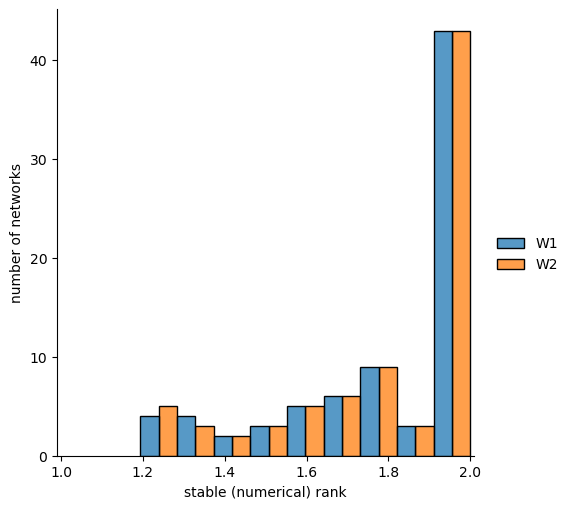
\includegraphics[scale=.45]{figures/final_f2s_displot.png}}
        \centering
        \caption{A histogram of the stable ranks at $0$-loss convergence.}
    \label{fig:empirical-high-f2s}
    \end{figure}
    
    \note{
        \footnotesize
        We saw that GF does not converge close~to low-rank~solutions for small enough initialization schemes, with some positive~probability. A simple experiment we conducted corroborates this and suggests that it holds with~high~probability for standard~initializations.
        \newline
        We consider the ``stable/numerical~rank" that approximates the standard~algebraic~rank. Intuitively, it measures the concentration of the singular values in the first singular value. Its image ranges between $1$ and the maximal standard~rank, which equals $2$ in our case. The stable rank equals~$1$ if~and~only~if the matrix has rank~$1$.
        \newline
        The figure is a histogram of the stable ranks of the two weight~matrices at convergence, $W1$ and $W2$, based on a few hundred repeats with a unique initialization. It counts the number of runs that converged to some stable rank.
        \newline
        The figure clearly suggests that whenever convergence to $0$~loss occurs, GD converges to networks with stable~ranks bounded~away from~$1$.
        \newline
        {   
            \tiny
            \alert{Setup:}
            ReLU networks; $W^{(1)},W^{(2)} \in \reals^{2 \times 2}$. \textbf{Dataset:} $\{(\bx_i,\by_i)\}_{i=1}^{2}$ ; $\by_1,\by_2$ are the standard~basis of~$\reals^2$; $\bx_1,\bx_2$ are~$(1,0.99), (-1,0.99)$ normalized to have unit~norm. \textbf{Initialization:} Every row of~$W^{(1)}$ and every column of~$W^{(2)}$ is drawn uniformly from the sphere of radius~$10^{-4}$ at the origin. \textbf{To simulate GF}: Do $3\cdot 10^{6}$~epochs of full-batch~GD of step~size~$10^{-4}$, w.r.t. the square~loss. Of~$288$~repeats, $79$~converged to \textbf{negligible~loss}~(defined~as~$<10^{-4}$).
        }
    }
\end{frame}



\begin{frame}{Proof ideas I}
    Recall:
    \pause
    \begin{assumption}
        The two target~vectors~$\by_1, \by_2$ are on the unit~sphere~$\mathbb{S}^1$ and are linearly~independent.
    \end{assumption}
    \begin{assumption}
        The two inputs~$\bx_1, \bx_2$ are on the unit~sphere~$\mathbb{S}^1$ and $\frac{\pi}{2} < \measuredangle(\bx_1, \bx_2) < \pi$.
    \end{assumption}
    \begin{exampleblock}{Thm. \hfill\checkmark}\label{T2}
        Let $(X,Y) \in \mathbb{R}^{2 \times 2} \times \mathbb{R}^{2 \times 2}$ be a labeled dataset that satisfies Assumptions~\ref{assumption:ys_linearly_independent},~\ref{assumption:xs_bounded_angle}.
        Consider GF w.r.t. the square~loss~$L_{X,Y}(W,V)$. Suppose that $W,V \in \reals^{2 \times 2}$ are initialized s.t. 
        $\norm{\bw_i(0)} < \min \left\{ \frac{1}{2}, \frac{\sqrt{3}}{2} \cos{\frac{\measuredangle(\bx_1, \bx_2)}{2}} \right\}$ 
        and $\norm{\bv_i(0)} < \frac{1}{2}$ for all $i \in \{1,2\}$. If GF converges to a $0$-loss~solution~$N_{W(\infty),V(\infty)}$, then $\rank W(\infty) = 2$.
    \end{exampleblock}
    
    \note{
        Now, to the main ideas in the proofs. I~will briefly remind the first statement.
        \begin{enumerate}
            \item We have a training dataset on the unit sphere: Two linearly~independent target~vectors, denoted by~$\by_i$, and two input~vectors having an obtuse~angle between them,~$\bx_i$. We initialize two weight~matrices~$W,V$ that parameterize a depth-$2$~ReLU~network s.t. the rows of~$W$, which we denote by~$\bw_i$, and the columns of~$V$, marked by~$\bv_i$, are all small. The guarantee is that if GF converges to a $0$-loss~solution, then $W(\infty)$ is full-ranked. In other words, the network at~convergence is full-ranked.
        \end{enumerate}
        The proof begins with defining four non-empty~regions that split the 2D~plain.
    }
\end{frame}



\begin{frame}
    \begin{columns}
            \begin{column}{0.5\textwidth}
                \begin{figure}[t]
                    \centering
                    \frame{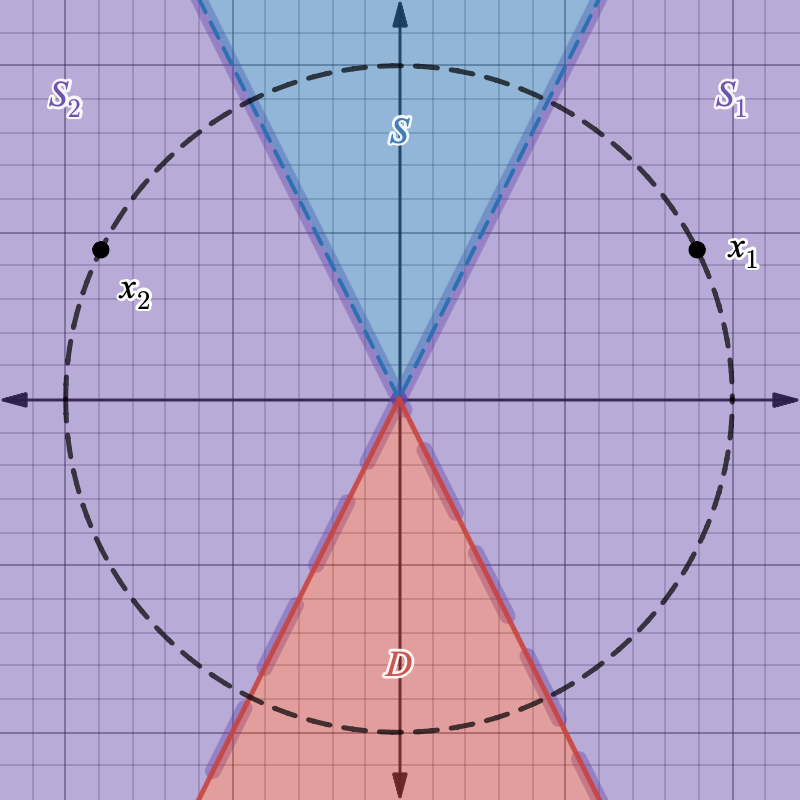
\includegraphics[scale=.24]{figures/D_and_Ss_regions.png}}
                    \caption{Regions $\cd, \cs, \cs_1, \cs_2$.}
                    \label{fig:D_and_Ss_regions}
                \end{figure}
            \end{column}
            \pause
            
            \begin{column}{0.7\textwidth}
                {\fontsize{10}{10} \selectfont
                \begin{eqnarray*}
                    &\mathcal{D} := \{ \bw \mid \forall i \in [2], \sigma(\bw^\top \bx_i) \le 0\}\\
                    \pause
                    &\mathcal{S} := \{ \bw \mid \forall i \in [2], \sigma(\bw^\top \bx_i) > 0 \}\\
                    \pause
                    &\mathcal{S}_j := \{ \bw  \mid  i=j \Leftrightarrow \sigma(\bw^\top \bx_i) > 0 \}
                \end{eqnarray*}
                }
            \end{column}
    \end{columns}
    
    \note{
        \footnotesize
        The figure depicts the 2D plain, the given input vectors $\bx_1, \bx_2$ on the unit sphere, and the following four regions $\cd, \cs, \cs_1, \cs_2$.
        \begin{enumerate}
            \item Intuitively, $\cd$~defines the ``dead''~region where neurons output~$0$ on both~$\bx_1,\bx_2$. 
            \item $\cs$~is the ``active''~region where neurons have a positive~output on both~$\bx_1,\bx_2$. 
            \item $\cs_1,\cs_2$~are the ``partially~active''~regions, where neurons are active for only the corresponding input. It means, for example, that each neuron in $\cs_1$ is positively correlated with $\bx_1$ and non-positively correlated with $\bx_2$.
        \end{enumerate}
    }
\end{frame}



\begin{frame}
    \begin{columns}
        \begin{column}{0.6\textwidth}
            \begin{itemize}[<+->]
                \item Assume towards~contradiction: GF converges to some 0-loss~network $N_{W(\infty),V(\infty)}$ s.t. $\rank(W(\infty))<2$.
                \item 0-loss $\Rightarrow Y = V(\infty) \sigma \left( W(\infty) X \right)$.
                \item $\Rightarrow$ 
                \begin{align*}
                    2 &= \rank(Y) = \rank \left( V(\infty) \sigma \left(W(\infty) X \right) \right) \\
                    &\leq \rank \left( \sigma \left( W(\infty) X \right) \right).
                \end{align*}
            \end{itemize}
        \end{column}
        
        \onslide<0->{
            \begin{column}{0.4\textwidth}
                \begin{center}
                    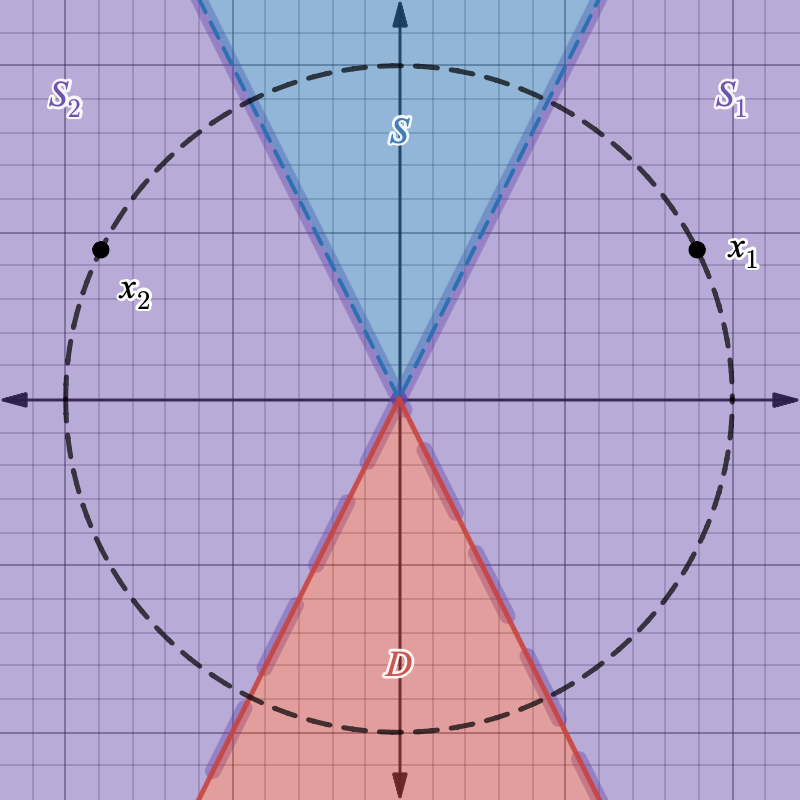
\includegraphics[width=\textwidth]{figures/D_and_Ss_regions.png}
                \end{center}
            \end{column}
        }
    \end{columns}
    
    \begin{itemize}
        \pause
        \item $\Rightarrow \bw_1(\infty), \bw_2(\infty) \notin \cd$. (Otherwise, $\zero^T$ is a row in~$\sigma(W(\infty) X)$.)
        \pause
        \item $\Rightarrow \bw_1(\infty), \bw_2(\infty) \ne \zero$ $\Rightarrow \rank(W(\infty))=1$. 
        \pause
        \item Denote $\bw_2(\infty) = \alpha \bw_1(\infty)$ where~$\alpha \neq 0$.
        \pause
        \begin{itemize}
            \item $\alpha > 0 \Rightarrow \sigma(\bw_2(\infty)^\top \bx_j) = \alpha \sigma(\bw_1(\infty)^\top \bx_j), \forall j \in [2] \Rightarrow$ contradiction!
            \item $\Rightarrow \alpha < 0$.
        \end{itemize}
        \pause
        \item $\Rightarrow$ W.l.o.g., $\bw_1(\infty) \in \cs_1 \setminus \partial \cs_1, \bw_2(\infty) \in \cs_2 \setminus \partial \cs_2$.
    \end{itemize}
    
    \note{
        \footnotesize
        Assume towards~contradiction that GF converges to some $0$-loss~network~$N_{W(\infty),V(\infty)}$ where~$\rank(W(\infty))<2$.
        \begin{enumerate}
            \itemsep=0pt
            \topsep=0pt
            \item The $0$-loss assumption means that the output of the network, $V(\infty) \sigma(W(\infty)X)$, equals the targets, $Y$.
            \item Since the targets are linearly independent, the rank of both sides equals~$2$. It implies that the output of the first layer, $\sigma(W(\infty)X)$ is full-ranked.
            \item
            \item Therefore, the weight~vectors~$\bw_1(\infty)$ and~$\bw_2(\infty)$ are~not in region~$\cd$. Otherwise, at~least one of the rows of~$\sigma(W(\infty) X)$ is~$\zero$, in~contradiction.
            \item In~particular, it implies that~$\bw_1(\infty)$ and~$\bw_2(\infty)$ are non-zero.\\
            By our first assumption that $\rank(W(\infty))<2$, we can conclude that its rank equals $1$ ((N.T.:~$\rank(W(\infty))=1$)).
            \item We denote~$\bw_2(\infty) = \alpha \bw_1(\infty)$ where $\alpha$ is non-zero.
            \item Note that if $\alpha$ was~positive, we could move it outside the ReLU. Then, the output~matrix of the first~layer,~$\sigma(W(\infty)X)$, would have its two rows linearly dependent, contradicting what we showed (i.e., that it is full-ranked). Therefore, $\alpha$ is strictly negative.
            \item Since we also have~$\bw_1(\infty),\bw_2(\infty) \not \in \cd$, then one of these weight~vectors is in interior~of~$\cs_1$ and the other is in interior~of~$\cs_2$. W.l.o.g., $\bw_j(\infty)$ is in the interior of $\cs_j$.
        \end{enumerate}
    }
\end{frame}




\begin{frame}
    We saw: $\bw_i(\infty) \in \cs_i \setminus \partial \cs_i$, and $\bw_2(\infty) = \alpha \bw_1(\infty)$ where $\alpha \neq 0$.
    \begin{columns}
        \begin{column}{0.55\textwidth}
            \pause
            \begin{itemize}[<+->]
                \item $\bw_i(t) \not\in \cd, \forall t$. (Otherwise, $\frac{d}{dt}~\bw_i(t)=\zero, \forall t : \bw_i(t) \in \cd$ $\Rightarrow \bw_i(\infty) \in \cd$ in contradiction.)
                \item $\bw_i(t) \in \cs_i \Rightarrow \frac{d}{dt} \bw_i(t) \in \spn\{\bx_i\}$.
                \item $t_i' := \inf \{t \mid \bw_i(t') \in \mathcal{S}_i, \forall t' \geq t\}$.
                \item $\Rightarrow \frac{d}{dt} \bw_i(t) \in \spn\{\bx_i\}, \forall t \geq t_i'$.
                \item $\Rightarrow \bw_i(\infty) \in \ca_i$.
                \item Show: $\bw_i(\infty) \in \cf_i$. $\Rightarrow \bw_2(\infty) \ne \alpha \bw_1(\infty)$!
            \end{itemize}
        \end{column}

        \begin{column}{0.45\textwidth}
            \begin{center}
                \includegraphics<handout:0|1-5>[width=\textwidth]{figures/D_and_Ss_regions.png}%
                \includegraphics<6->[width=\textwidth]{figures/F_and_A_regions.png}%
            \end{center}
        \end{column}
    \end{columns}
    
    \note{
        \footnotesize
        By observing the gradients of the loss function w.r.t.~$\bw_i$, the following facts follow for all $i$.
        \begin{enumerate}
            \itemsep=0pt
            \topsep=0pt
            \item First, if~$\bw_i \in \cd$ at some time~$t$, then its derivative equals $\zero$. Hence, $\bw_i$~remains at~$\cd$ indefinitely, so it does not converge in the interior of $\cs_i$, in~contradiction. Thus, the trajectory~$\bw_i(t)$ does~not visit~$\cd$.
            \item Second, if~$\bw_i \in \cs_i$ at time~$t$, then $\bx_i$ spans its derivative.
            \item Since~$\bw_i(\infty)$ is in the interior of $\cs_i$, we can consider the last~time~$t_i'$ that~$\bw_i$ enters~$\cs_i$. It can be either at the initialization (i.e.,~$t_i'=0$) or when moving from~$\cs$ (i.e.,~$t_i'>0$).
            \item For~all time~$t$ at~$t_i'$~or~later, we have that the derivative of $\bw_i$ is in the span of $\bx_i$.
            \item It allows us to conclude that~$\bw_i(\infty)$ must be in the region~$\ca_i$ that you see in the figure. (It is the union of the orange and green regions.)
            \item Lastly, we show a lower bound on~$\norm{\bw_i(\infty)}$ so that $\bw_i(\infty)$ is in region~$\cf_i$ as in the figure. Then, we have $\bw_1(\infty) \in \cf_1$ and $\bw_2(\infty) \in \cf_2$, implying that the angle between the neurons must be smaller than $\pi$, in~contradiction to $\bw_2(\infty) = \alpha \bw_1(\infty)$.
        \end{enumerate}
    }
\end{frame}




\begin{frame}
    We saw: $\bw_i(\infty) \in \ca_i$, and $\bw_2(\infty) = \alpha \bw_1(\infty)$ where $\alpha \neq 0$.\\
    Show: $\norm{\bw_i(\infty)}$ cannot be too~small. ($\Rightarrow \bw_i(\infty) \in \cf_i$.)
    \pause
    \begin{itemize}[<+->]
        \item \cite{du2018algorithmic}: $\norm{\bw_i(t)}^2 - \norm{\bv_i(t)}^2$ is constant.
        \begin{itemize}[<+->]
            \item $\norm{\bv_i(\infty)}$ is small $\Leftrightarrow \norm{\bw_i(\infty)}$ is small. ($\norm{\bw_i(0)}, \norm{\bv_i(0)}$ are small)
        \end{itemize}
    \end{itemize}
    \begin{columns}[T]
        \begin{column}{0.55\textwidth}
            \begin{itemize}[<+->]
                
                \item $0$~loss and~$\bw_i(\infty) \in \cs_i$ $\Rightarrow \by_i = \bv_i(\infty) (\bw_i(\infty)^\top \bx_i)$.
                \item Recall that $\norm{\by_i}=\norm{\bx_i}=1$.
                \item $\Rightarrow \norm{\bw_i(\infty)}, \norm{\bv_i(\infty)}$ are not both small.
            \end{itemize}
        \end{column}

        \begin{column}{0.45\textwidth}
            \begin{center}
                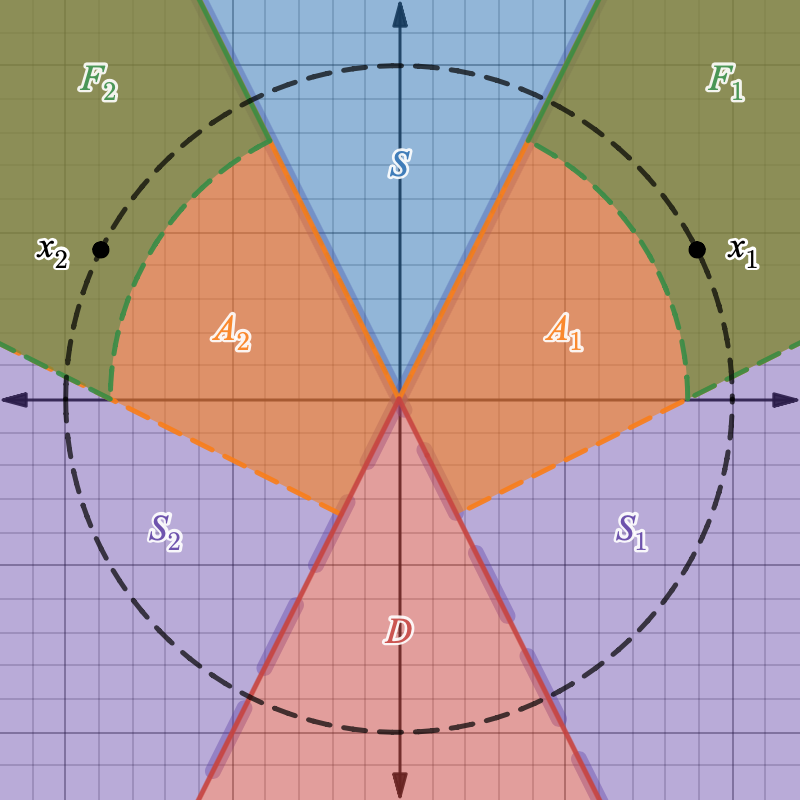
\includegraphics[width=\textwidth]{figures/F_and_A_regions.png}%
            \end{center}
        \end{column}
    \end{columns}
    
    \note{
        \footnotesize
        Informally speaking, we prove that $\bw_i(\infty) \in \cf_i$ by showing that $\norm{\bw_i(\infty)}$ cannot be too~small. 
        \begin{enumerate}
            \itemsep=0pt
            \topsep=0pt
            \item To do so, we apply a theorem from \cite{du2018algorithmic} that guarantees that the difference in the squared norms of $\bw_i$ and $\bv_i$ remains constant throughout the training. Namely, for all $t$.
            \item Recall that, at the initialization, the norms of both~$\bw_i$ and~$\bv_i$ are small. The consequence is that, also at convergence, their norms have only a small difference between them. Hence, at convergence, the norm of $\bv_i$ is~small if~and~only~if the norm of $\bw_i$ is~small.
            \item Since the network attains $0$~loss and~$\bw_i(\infty) \in \cs_i$ for~all~$i$, then the following equation holds. Namely, the output of the network is determined only by the $i$-th~neuron, and it equals the target, $\by_i$.
            \item Recall our assumption that the inputs and targets lie on the unit sphere.
            \item It implies that it is impossible that, at convergence, both $\bw_i$ and $\bv_i$ are small.
        \end{enumerate}
        The lower bound on~$\norm{\bw_i(\infty)}$ follows, and it completes the proof.
    }
\end{frame}




\begin{frame}
    \begin{exampleblock}{Thm. \hfill\checkmark} \label{T3}
        Let $(X,Y) \in \mathbb{R}^{2 \times 2} \times \mathbb{R}^{2 \times 2}$ be a labeled dataset that satisfies Assumptions~\ref{assumption:ys_linearly_independent} and~\ref{assumption:xs_bounded_angle}.
        Consider GF w.r.t. the square loss~function $L_{X,Y}(W,V)$. Suppose that $W,V \in \reals^{2 \times 2}$ are initialized s.t. for all $i \in \{1,2\}$ we have $\bv_i(0) = \zero$, and $\bw_i(0)$ is drawn from a spherically~symmetric distribution with 
        \begin{align*}
            \norm{\bw_i(0)} 
            \leq \frac{\sqrt{3}}{2} \min \left\{ 
            \sin\left(\frac{\pi - \measuredangle(\bx_1,\bx_2)}{4} \right), 
            \sin \left(\measuredangle(\bx_1,\bx_2) - \frac{\pi}{2}\right)
            \right\} ~.
        \end{align*}
        Let $E$ be the event that GF converges to a 0-loss~solution~$N_{W(\infty),V(\infty)}$ s.t.
        \begin{itemize}
            \item[(i)] $\measuredangle \left( \bw_1(\infty), \bw_2(\infty) \right) \in \left[ \frac{\pi}{2} - \left(\measuredangle(\bx_1, \bx_2) - \frac{\pi}{2} \right), \frac{3\pi}{4} + \frac{\measuredangle(\bx_1, \bx_2) - \pi/2}{2} \right]$,
            \item[(ii)] $\norm{\bw_i(\infty)} \in \left( \frac{\sqrt{3}}{2}, \sqrt{ \frac{1}{4} + \frac{4}{3 \left(\sin \measuredangle(\bx_1, \bx_2) \right)^2 } } \right)$ for all $i \in \set{1, 2}$.
        \end{itemize}
        Then, $\Pr \left[E \right] \ge 2 \cdot \left(\frac{\measuredangle(\bx_1,\bx_2)}{2\pi} \right)^2$.
    \end{exampleblock}
    
    \note{
        \footnotesize
        This theorem (that we already introduced) has much in common with what we just saw. The statement is now probabilistic over the randomness of the initialization and holds the same assumptions on the dataset: The inputs and targets lie on the unit sphere, the targets are linearly independent, and the angle between the inputs is obtuse. The guarantee is that, with positive probability, small enough random~initializations lead to high~ranks for any rank-approximation~metric. Specifically, we assure that, at~convergence, the norm of the hidden~neurons, $\bw_1, \bw_2$, is in~a~bounded~interval, as~well~as the angle~between~them.\\
        The main~difference from the previous~theorem is that now we consider rank-approximation like the stable/essential~rank. To guarantee that any such~rank~approximation is~bounded~away~from~$1$, it is necessary to~bound the norms~and~angle.
    }
\end{frame}




\begin{frame}{Proof ideas II}
    If $\bw_1(0) \in \cs_1 \setminus \partial \cs_1, \bw_2(0) \in \cs_2 \setminus \partial \cs_2$:
    \begin{columns}[T]
        \begin{column}{0.55\textwidth}
            \begin{itemize}[<+->]
                \item $\forall t:$
                \begin{enumerate}
                    \item $\frac{d}{dt} \bw_i(t) = C_i(t) \bx_i, C_i(t) \geq 0$.
                    \item $\bw_i(t) \in \cs_i \setminus \partial \cs_i$.
                \end{enumerate}
                \item $\Rightarrow$ $N_{W(\infty),V(\infty)}$ exists with $0$ loss.
                \item $\Rightarrow \bw_i(\infty) \in \cf_i$.
                \item Recall: $\bw_i(0) \sim$ some~spherically symmetric distribution.
                \item $\Rightarrow$ $\Pr \left[ \forall i : \bw_i(0) \in \cs_i \setminus \partial \cs_i \right] \ge 2 \cdot \left(\frac{\measuredangle(\bx_1,\bx_2)}{2\pi} \right)^2$.
                \hfill\qedsymbol
            \end{itemize}
        \end{column}

        \begin{column}{0.45\textwidth}
            \begin{center}
                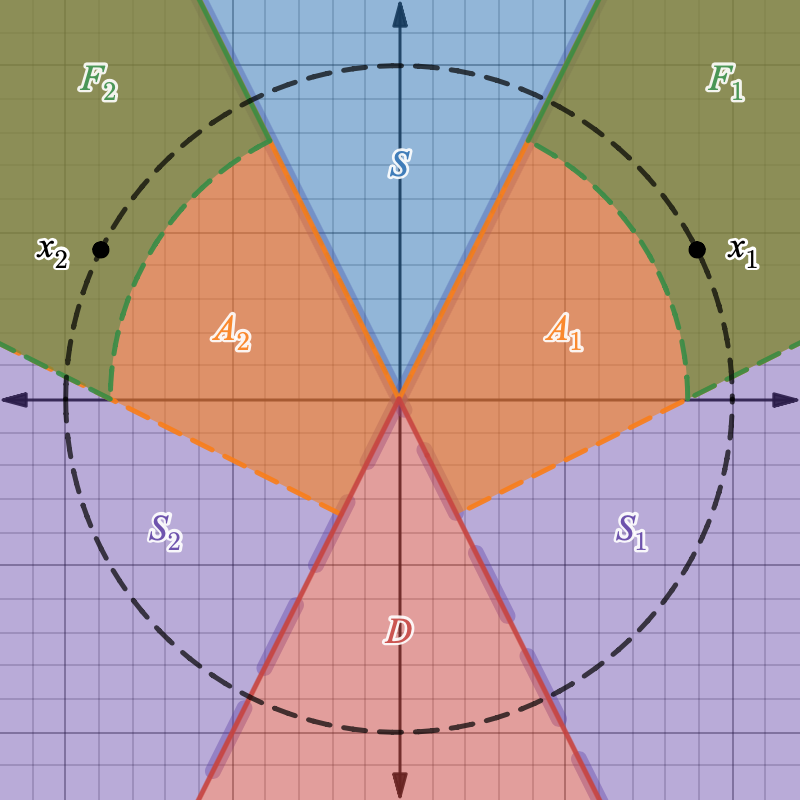
\includegraphics[width=\textwidth]{figures/F_and_A_regions.png}%
            \end{center}
        \end{column}
    \end{columns}
    
    \note{
        \footnotesize
        The key analysis in the proof is of the dynamics where $\bw_i$ is in the interior of $\cs_i$, for all $i$. Suppose that, at initialization, we have $\bw_i(0)$ is in the interior of $\cs_i$, for all $i$.
        \begin{enumerate}
            \item Then, it is possible to show that the dynamics are such that: (1) $\bw_i$ moves towards $\bx_i$ until convergence, and
            \item (2) $\bw_i$ never leaves the interior of $\cs_i$.
            \item We prove that these properties of the hidden neurons trajectory imply that GF converges to a $0$-loss~network.
            \item Similar to what we saw for the previous theorem, we complete by proving that $\bw_i(\infty) \in \cf_i$.\\
            Therefore, it is sufficient to argue that $\bw_i$ is in the interior of $\cs_i$ at initialization.
            \item Recall that the distribution of the random initialization of the hidden neurons is spherically symmetric.
            \item Hence, simple geometric arguments allow us to bound the probability that the hidden~neurons initially lie in the interiors as required. The exact lower~bound depends only on the angle~between~the~two~inputs.
        \end{enumerate}
    }
\end{frame}



\begin{frame}{Our results}{Rank~min. in deep~networks with small~$\ell_2$~norm}
    \pause
    Settings: ReLU~networks, overparameterized in \true{depth}, of width $\ge 2$, trained with the square~loss.
    \pause
    \begin{exampleblock}{Thm. (informal)}
        For sufficiently deep networks, if $\btheta(\infty)$ exists and $\btheta(\infty) \in \arg\min_{\btheta} \norm{\btheta}$ s.t. $L_{X,Y}(\btheta(\infty)) = 0$, then 
        \[
        \frac{1}{k}\sum_{i=1}^{k} \frac{\norm{W^{(i)}(\infty)}_\sigma}{\norm{W^{(i)}(\infty)}_F}
        \approx 1
        \]
    \end{exampleblock}
    \pause
    \begin{itemize}
        \item The \emph{stable~rank} of $W := {\norm{W}^2_F} / {\norm{W}^2_\sigma}$.
        \pause
        \item $\Rightarrow$ There is a bias towards \true{low~ranks}.
        \pause
        \item GF is \alert{not}~known to be biased to minimize the $\ell_2$ norm.
        \pause
        \item In practice: Commonly use explicit $\ell_2$ regularization, which encourages norm~minimization.
    \end{itemize}
    
    \note{
        \footnotesize
        For ReLU~networks that are overparameterized in~terms of depth and have width~$\ge 2$, we identify settings in which GF \textbf{is} biased towards low~ranks.
        \begin{enumerate}
            \itemsep=0pt
            \topsep=0pt
            \item First, we consider ReLU~networks trained w.r.t. the square~loss.
            \item We show that for sufficiently deep networks, if GF converges to a network that attains $0$~loss and minimizes the $\ell_2$-norm~of~the~parameters, then the average~ratio between the spectral and the Frobenius~norms of the weight~matrices is close~to~$1$.
            \item The squared inverse of this ratio is known~as the \emph{stable~rank}. It is a continuous~approximation of the rank.\\
            The ratio of spectral-to-Frobenius~norms of some matrix~$W$ and the inverse of this ratio have both the following important property: They equal~$1$ if~and~only~if $\rank(W)$ is~$1$.
            \item Therefore, our result reveals a bias towards low~ranks.
            \item A possible critique on the statement of the theorem might be: ``Why assume that $\norm{\btheta}$ is minimal? GF in ReLU~networks w.r.t. the square~loss is \textbf{not}~known to be biased towards solutions that minimize the $\ell_2$~norm."
            \item While this is generally true, in practice, it is common to use explicit $\ell_2$-regularization, which encourages norm~minimization. Thus, our result suggests that GF in deep networks trained with the square~loss and explicit $\ell_2$-regularization encourages rank~minimization.
        \end{enumerate}
    }
\end{frame}




\begin{frame}
    \begin{exampleblock}{Thm. \hfill\checkmark}
        Let~$\left\{ \left( \bx_i, y_i \right) \right\}_{i=1}^n \subseteq \mathbb{R}^{\din} \times \reals_+$ s.t. $\exists i \in [n]$ satisfying~$\norm{\bx_i} \leq 1$ and $y_i \geq 1$. 
        \pause
        Assume that $\exists N$, a fully-connected~neural~network of width~$m \geq 2$ and depth~$k \geq 2$, s.t. $\forall i \in [n]$ we have~$N(\bx_i) = y_i$, and the weight matrices $W_1,\ldots,W_k$ of $N$ satisfy $\norm{W_i}_F \leq B$ for some~$B>0$.
        \pause
        Let~$N_\btheta$ be a fully-connected~neural~network of width~$m' \geq m$ and depth~$k' > k$ parameterized by~$\btheta$.
        \pause
        Let~$\btheta^* = \left[W_1^*,\ldots,W_{k'}^*\right]$ be a global~optimum of the following problem: $\min_\btheta \norm{\btheta} \;\;\;\; \text{s.t. } \;\;\; \forall i \in [n] \;\; N_\btheta(\bx_i)=y_i$.
        \pause
        Then, 
        \setcounter{equation}{0}
        {\setlength{\abovedisplayskip}{0pt}
        \setlength{\belowdisplayskip}{0pt}
        \begin{equation}  \label{eq:average ratio square}
            \frac{1}{k'}\sum_{i=1}^{k'} \frac{\norm{W_i^*}_\sigma}{\norm{W_i^*}_F} 
            \geq \left( \frac{1}{B} \right)^{\frac{k}{k'}}~.
        \end{equation}
        Equivalently,
        \begin{equation}  \label{eq:harmonic ratio square}
            \frac{k'}{\mathlarger{\sum}_{i=1}^{k'} \left( \frac{\norm{W_i^*}_F}{\norm{W_i^*}_\sigma} \right)^{-1} }
            \leq 
            B^{\frac{k}{k'}}~.
        \end{equation}
        }
    \end{exampleblock}
    \pause
    \begin{itemize}
        \item If $k' >> k$: The RHS of \eqref{eq:average ratio square} and \eqref{eq:harmonic ratio square} is roughly~$1$. 
        \pause
        $\Rightarrow$ \true{low rank}.
        \pause
        \item Does~not depend on the width of either network or the rank of $N$.
    \end{itemize}
    
    \note{
        \scriptsize
        I will present the formal statement of the theorem step by step.\\
        First, we assume that the dataset consists of input vectors with a corresponding positive~scalar~target, such that there exists at least one input-output pair having their norms at~most and at~least~$1$, respectively.
        \begin{enumerate}
            \itemsep=0pt
            \topsep=0pt
            \item We assume that there~exists a fully-connected~neural~network~$N$ of width~and~depth at~least~$2$, that attains $0$ loss, and its weight~matrices have their Frobenius norm uniformly bounded by some constant B.
            \item We define a new fully-connected~neural~network, denoted by~$N_\btheta$, which is deeper than~$N$ and possibly wider.
            \item $\btheta^*$ is a $0$-loss parameterization of $N_\btheta$ with minimal norm.
            \item The guarantee is that the average ratio of spectral~to~Frobenius~norm is lower~bounded. Equivalently, the harmonic mean of the Frobenius~to~spectral~norm~ratio is upper~bounded.
            \item Hence, if $k'$ is much larger than $k$, namely, $N_\btheta$ is much deeper than $N$, than the right-hand side in both expressions, \eqref{eq:average ratio square} and \eqref{eq:harmonic ratio square}, is roughly~$1$.
            \item These two ratios in \eqref{eq:average ratio square} and \eqref{eq:harmonic ratio square}, namely, the spectral-to-Frobenius and  Frobenius-to-spectral, equal~$1$ if~and~only~if the matrix is of rank~$1$. Therefore, there is a bias towards low-rank~solutions as the depth~$k'$ increases.
            \item Note that the result does~not depend on the width of the networks. That is, even if we train an extremely~wide network, the bias towards low~ranks exists as~long~as its depth,~$k'$, is~large. Also, the theorem holds even if the network~$N$ has high~ranks (e.g., all its weight~matrices are full-ranked). By the theorem, once we consider deep enough networks, the dataset becomes realizable even by a network of small average~rank, and GF converges to such a network.
        \end{enumerate}
    }
\end{frame}



\begin{frame}{Proof idea}
    \begin{itemize}[<+->]
        \item Suppose $\exists$ a $0$-loss network s.t. each layer has Frobenius~norm~$B$.
        \item $\Rightarrow \exists$ a deeper $0$-loss network $N_\btheta$ s.t. each layer has Frobenius~norm~$B^* << B$. ($B^* \lessapprox 1$)
        \item $\exists i \in [n]$ s.t. $\norm{\bx_i} \leq 1, y_i \geq 1$. $\Rightarrow N_\btheta(\bx_i) \ge 1$.
        \item $\Rightarrow$ The average~spectral~norm of the layers in $N_\btheta$ is $\ge 1$.
        \item $\Rightarrow$ The average ratio of spectral-to-Frobenius~norms in $N_\btheta$ cannot be too small.
    \end{itemize}
    
    \note{
        \footnotesize
        At a very high level, the idea of the proof is the following: On the one hand, upper~bounding the Frobenius norm of the layers in $N_\theta$. On the other hand, lower~bounding the average spectral norm.\\
        We start by assuming that the dataset is realizable by some network such that the Frobenius~norm of each of its weight~matrices equals~$B$.
        \begin{enumerate}
            \itemsep=0pt
            \topsep=0pt
            \item We show that the dataset is also realizable by a deeper~network, $N_\btheta$, where the Frobenius~norm of each layer is~$B^*$, while~$B^*$ is much~smaller than~$B$. Moreover, if the network is sufficiently~deep, then~$B^*$ is~not much~larger than~$1$.
            \item On the other hand, we lower~bound the spectral~norm in~$N_\theta$. Recall that we assumed to have an input of norm at~most~$1$ with a corresponding target of size at~least~$1$. Since $N_\theta$ attains $0$ loss, the output of the network for this input is also of size at~least~$1$.
            \item Therefore, the average~spectral~norm of the layers is at~least~$1$.
            \item It allows us to complete the proof by concluding that the average~ratio between the spectral and Frobenius~norms cannot be too small.
        \end{enumerate}
        The main trick here hides in our claim that $N_\btheta$~exists. Namely, a $0$-loss network that all its layers have Frobenius~norm~$B^*$, which is almost~$1$.\\
        The following construction proves it.
    }
\end{frame}




\begin{frame}
    Assume: $\exists N$ of width~$m$, depth~$k$, $0$ loss, Frobenius~norm~$B$ in all layers.\\
    Construct: $N'$ of width~$m$, depth~$k' > k$, $0$ loss, Frobenius~norm~$B^* \lessapprox 1$ in all layers.
    \pause
    \begin{itemize}
        \item $\forall i \in [k], W'_i := \alpha W_i$ where $\alpha = \left( \frac{1}{B} \right)^{\frac{k'-k}{k'}}$.
        \pause
        \item $\forall i \in \set{k, k+1, \ldots, k'}, W'_i \in \reals$.
        \pause
        \item $\forall i \in \set{k+1, \ldots, k'}, W'_i := \beta$, where $\beta = \left( \frac{1}{B} \right)^{-\frac{k}{k'}}$.
        \pause
        \item $\Rightarrow N'(\bx_i) = N(\bx_i) \cdot \alpha^k \cdot \beta^{k'-k} = N(\bx_i)$. 
        \pause
        $\Rightarrow N'$ has $0$ loss.
        \pause
        \item Let $\btheta^* = \left[W^*_1,\ldots,W^*_{k'} \right] \in \min_\btheta \norm{\btheta} \text{ s.t. } \forall i \in [n], N_\btheta(\bx_i)=y_i$.
        \pause
        \item $\Rightarrow B^* = \norm{W^*_i}_F = \norm{W^*_j}_F, \forall i, j \in [k']$.
        \pause
        \item $\norm{\btheta^*} \leq \norm{\btheta'} \Rightarrow$ By calculation, $B^* \leq B^{\frac{k}{k'}}$.
        \hfill\qedsymbol
    \end{itemize}
    
    \note{
        \footnotesize
        We use the given $0$-loss network~$N$ of width~$m$ and depth~$k$ to construct a deeper $0$-loss network,~$N'$, of width~$m$ and depth~$k'$ as follows.
        \begin{enumerate}
            \item The first~$k$~layers of~$N'$ are obtained by scaling the layers of~$N$ by a factor~$\alpha$.
            \item Since the output~dimension of~$N$ is~$1$, the $k$-th hidden~layer of~$N'$ has width~$1$. The rest of the layers in~$N'$ are also of width~$1$.
            \item The weight in each of these last $k'-k$ layers is~$\beta$.
            \item Therefore, given an input~$\bx_i$, the output of $N'$ equals the output of $N$. 
            \item In other words, $N'$ induces $0$ loss.
            \item Let~$\btheta^*$ be a $0$-loss parameterization with minimal $\ell_2$ norm.
            \item By the optimality of~$\btheta^*$, we show that its layers must be balanced. Namely, the Frobenius~norm of any pair of layers is equal. We denote the Frobenius~norm of the layers by~$B^*$.
            \item Since the norm of $\btheta^*$ is minimal, the parameterization of~$N'$, denoted by~$\btheta'$, cannot be smaller. Then, by a calculation, we can obtain the required upper~bound on~$B^*$. Note that as~long~as~$N_\btheta$ is~sufficiently~deep, namely, $k'$~is~large, then~$B^*$ cannot be much~greater~than~$1$, as~required.
        \end{enumerate}
    }
\end{frame}



\AtBeginSection[]
{
    \begin{frame}{Table of Contents}
        \tableofcontents[currentsection]
    \end{frame}
    
    \note{
        \footnotesize
        The last part of our work is about ReLU~networks in binary~classification~problems. We start with some additional,~necessary~preliminaries.
    }
}



\section{Classification}
\subsection{Preliminaries}

\begin{frame}{Preliminaries}{Implicit bias in \textbf{exponentially-tailed~losses}}
    \begin{definition}[classification loss]
        Given a binary~classification dataset $\{(\bx_i,y_i)\}_{i=1}^n \subseteq \reals^d \times \set{\pm 1}$, a network $N_\btheta$ and a loss function $\ell:\reals \to \reals$,
        \begin{equation*}\label{eq:objective classification}
        	L_{X,\by}(\btheta) := \sum_{i=1}^n \ell\left(y_i N_\btheta(\bx_i)\right)~.
        \end{equation*}
    \end{definition}
    \pause
    \begin{description}
        \item[exponential~loss] \, $\ell(q) := e^{-q}$.
        \item[logistic~loss] \, \, \, \, \, $\ell(q) := \log(1+e^{-q})$.
    \end{description}
    \pause
    \newline
    \newline
    \begin{itemize}
        \item $N_\btheta$ \emph{correctly~classifying} a dataset if $y_i N_\btheta(\bx_i) > 0, \forall i \in [n]$.
        \pause
        \item A~trajectory~$\btheta(t)$~of~GF {\em converges~in~direction}~to~$\tilde{\btheta}$ if 
        \[
            \lim_{t \to \infty}\frac{\btheta(t)}{\norm{\btheta(t)}} = \frac{\tilde{\btheta}}{\snorm{\tilde{\btheta}}}
        \]
    \end{itemize}
    
    \note{
        \footnotesize
        In this setting of binary~classification, the output~dimension of the network equals~$1$, and we consider empirical~classification~losses that are exponentially~tailed.
        \begin{enumerate}
            \item We focus on the exponential~loss and the logistic~loss.
            \item We say that a given dataset is \emph{correctly~classified} by the network~$N_\btheta$ if the inner~product of the~prediction~of~the~network and the~target is~positive for all inputs.
            \item We say that a~trajectory~$\btheta(t)$~of~GF {\em converges~in~direction} if the limit as~$t \to \infty$ of the~direction~of~$\btheta(t)$ exists.\\
            Note that with exponentially-tailed losses, $\norm{\btheta(t)} \to \infty$ as $t \to \infty$. Therefore, the emph{convergence~in~direction} is the only notation~of~converges in this~setting.
        \end{enumerate}
    }
\end{frame}



\subsection{Previous work}
\begin{frame}{Previous work}{Implicit bias in linear~networks with exponentially-tailed~losses}
    % NOTE: \cite{soudry2018implicit} is less relevant comparing to the following prior results 
    % \begin{exampleblock}{\cite{soudry2018implicit}}
    %      GD on linearly-separable~binary~classification~problems converges to the maximum~$\ell_2$-margin~direction.
    % \end{exampleblock}
    % \pause
    % \begin{itemize}
    %     \item Extended to other loss~functions, tighter convergence~rates, non-separable~data, and variants of gradient-based~optimization~algorithms \citep{nacson2019convergence,ji2018risk,ji2020gradient,gunasekar2018characterizing,shamir2021gradient,ji2021characterizing}.
    % \end{itemize}
    \pause
    \begin{exampleblock}{\cite{ji2018gradient, ji2020directional} \hfill\checkmark}
        In linear networks, GF converges s.t. every layer has rank~$1$, namely, $\rank W^{(i)}(\infty) = 1, ~\forall i \in [k]$.
    \end{exampleblock}
    \pause
    \begin{definition}[homogeneous neural network]
        $N_\btheta$~is~\emph{homogeneous} if $\exists M > 0$ s.t. $N_{\alpha \btheta}(\bx) = \alpha^M N_\btheta(\bx), \forall \btheta,\bx$ and $\alpha>0$.
    \end{definition}
    \pause
    \begin{itemize}
        \item ReLU networks are homogeneous.
    \end{itemize}
    \pause
    \begin{exampleblock}{\cite{lyu2019gradient,ji2020directional} (informal) \hfill\checkmark}
          In homogeneous~networks, GF converges~in~direction to a KKT~point of the maximum~$\ell_2$-margin~problem in the parameter~space.
    \end{exampleblock}
    \pause
    \begin{exampleblock}{Thm. (informal)}
        For sufficiently~deep~networks, maximizing~the~$\ell_2$-margin $\Rightarrow$ \true{rank~minimization}.
    \end{exampleblock}
    
    \note{
        \scriptsize
        \begin{enumerate}
            \item For linear networks of output~dimension~$1$, \cite{ji2018gradient, ji2020directional} showed that gradient~flow~(GF) w.r.t. exponentially-tailed~classification~losses converges to networks where the weight~matrix of every layer is of rank~$1$.
            \item In \emph{homogeneous}~neural~networks, like the ReLU networks, a well-known result characterizes the implicit~bias for the~logistic~or~the~exponential~losses.\\
            We say that a network~$N_\btheta$~is~\emph{homogeneous} if there~exists a~positive~constant~$M$ that satisfies the following. Multiplying any parameterization of the network,~$\btheta$, by a~positive~scalar,~$\alpha$, always results in just multiplying the prediction of the network by $\alpha^M$. 
            \item As mentioned, fully-connected~ReLU~networks are homogeneous.
            \item \cite{lyu2019gradient} and \cite{ji2020directional} showed that GF on homogeneous~neural~networks, with exponentially-tailed~losses, converges~in~direction to a KKT~point of the maximum-margin~problem in the parameter~space.\\
            It means that GF in such networks is biased towards networks that maximize~the~$\ell_2$-margin. 
            \item Our~result shows that for sufficiently~deep~networks, maximizing~the~margin implies rank~minimization, where the rank is measured by the~ratio~between~the~norms as~we~saw.
        \end{enumerate}
        We won't cover other prior works that studied the implicit~bias in diagonal and convolutional~linear~networks, as well as in infinitely-wide~homogeneous~networks.\\
        ((N.T: \cite{gunasekar2018bimplicit,moroshko2020implicit,yun2020unifying} \& \cite{chizat2020implicit}))
    }
\end{frame}




\begin{frame}
    \begin{exampleblock}{Paraphrased from \cite{lyu2019gradient,ji2020directional} \hfill\checkmark}
        \pause
        Let~$N_{\btheta}$ be a homogeneous~ReLU~neural~network.
        \pause
        Consider minimizing the average of either the exponential or the logistic~loss over a binary~classification dataset using~GF.
        \pause
        Suppose that the average~loss converges to zero as~$t \to \infty$.
        \pause
        Then, GF converges~in~direction to a first~order stationary~point (KKT~point) of the following maximum~margin~problem in parameter~space:
        \begin{equation*}
        \label{eq:optimization problem}
        	\min_\btheta \frac{1}{2} \norm{\btheta}^2 \;\;\;\; \text{s.t. } \;\;\; \forall i \in [n] \;\; y_i N_\btheta(\bx_i) \geq 1~.
        \end{equation*}
    \end{exampleblock}
        
    
    \note{
        \footnotesize
        We phrase the following lemma based on \cite{lyu2019gradient,ji2020directional}.
        \begin{enumerate}
            \item For a homogeneous~ReLU~neural~network,
            \item given a binary~classification dataset, GF minimizes the average of either the exponential or the logistic~loss.
            \item Assume that, eventually, the average~loss converges to~$0$.
            \item Then, GF converges~in~direction to a KKT~point of this maximum~margin~problem.\\
        \end{enumerate}
        This lemma suggests that GF tends to converge~in~direction to networks with margin~$1$ and small~$\ell_2$~norm.\\
        Our following theorem shows the~implication~of~the~lemma for deep~overparameterized~ReLU~networks. It guarantees that if GF converges~in~direction to an optimal~solution of this max-margin~problem, its layers tend to have low~rank.
    }
\end{frame}



\subsection{Our results}

\begin{frame}
    \begin{exampleblock}{Thm. \hfill\checkmark}
        \setlength{\abovedisplayskip}{0pt}
        \setlength{\belowdisplayskip}{0pt}
        \pause
        Let $\left\{ \left( \bx_i, y_i \right) \right\}_{i=1}^n \subseteq \mathbb{R}^{\din} \times \set{\pm 1}$ be a binary classification dataset, and assume that $\exists i \in [n]$ with $\norm{\bx_i} \leq 1$. 
        \pause
        Assume that $\exists$ a fully-connected neural network~$N$ of width~$m \geq 2$, depth~$k \geq 2$, s.t. $\forall i \in [n], y_i N(\bx_i) \geq 1$ and its weight matrices~$W_1,\ldots,W_k$ satisfy~$\norm{W_i}_F \leq B$ for some~$B>0$.
        \pause
        Let $N_\btheta$ be a fully-connected neural~network of width~$m' \geq m$, depth~$k' > k$, parameterized by~$\btheta$. 
        \pause
        Let~$\btheta^* = \left[W_1^*,\ldots,W_{k'}^*\right]$ be a global optimum of the maximum $\ell_2$-margin problem. Namely, $\btheta^*$ parameterizes a minimum-norm fully-connected network of width~$m'$, depth~$k'$, that labels the dataset correctly with margin~$1$.
        \pause
        Then,
        \begin{equation*} \label{eq:average ratio exp}
            \frac{1}{k'} \sum_{i=1}^{k'} \frac{\norm{W_i^*}_\sigma}{\norm{W_i^*}_F} \geq \frac{1}{\sqrt{2}} \cdot \left( \frac{\sqrt{2}}{B} \right)^{\frac{k}{k'}} \cdot \sqrt{\frac{k'}{k'+1}}
        \end{equation*}
        \pause
        Equivalently, 
        \begin{equation*} \label{eq:harmonic ratio exp}
            \frac{k'}{\mathlarger{\sum}_{i=1}^{k'} \left( \frac{\norm{W_i^*}_F}{\norm{W_i^*}_\sigma} \right)^{-1}}
            \leq \sqrt{2} \cdot \left( \frac{B}{\sqrt{2}} \right)^{\frac{k}{k'}} \cdot \sqrt{\frac{k'+1}{k'}}
        \end{equation*}
    \end{exampleblock}
    
    \note{
        \scriptsize
        \begin{enumerate}
            \item Let a binary~classification dataset consists of targets~$\pm 1$ and at~least~one input~vector of norm at~most~$1$.
            \item We assume that $N$ is a fully-connected~neural~network of width~and~depth of at~least~$2$ that correctly~classifies the dataset. Also, all the weight~matrices of $N$ are uniformly~bounded by some positive~constant~$B$.
            \item $N_\btheta$ is a deeper, fully-connected~neural~network that may also be wider than the~network~$N$.
            \item $\btheta^*$ is a parameterization of $N_\btheta$ that is also a global~optimum of the maximum-margin~problem~in~the~parameter~space we saw earlier. Namely, $\btheta^*$ is a minimal-norm~parameterization that correctly~classifies the dataset by a~margin~of~$1$.
            \item The guarantee is that the average~ratio of the spectral-to-Frobenius~norms is lower~bounded such~that whenever the depth~$k'$ of the trained network~$N_\btheta$ is sufficiently large, this average~ratio is at~least roughly~$1/\sqrt{2}$.
            \item Equivalently, we have the following upper~bound on the harmonic~mean of the Frobenius-to-spectral~ratios. As remembered, this ratio is the square~root of the stable~rank. For sufficiently large depth~$k'$, it is at~most roughly~$\sqrt{2}$.
        \end{enumerate}
        Note that the result does~not depend on the width~of~the~networks or their ranks, as in our previous~theorem.
    }
\end{frame}



\begin{frame}
    \pause
    \begin{itemize}
        \item \cite{lyu2019gradient,ji2020directional} + our Thm. $\Rightarrow$\\
        GF over overparameterized~deep~fully-connected~networks tends to converge~in~direction to networks with \true{low~ranks}.
        \pause
        \item In exponential/logistic~loss, if $\lim_{t \to \infty} \text{loss} = 0 \Rightarrow \norm{\btheta(t)} \to \infty$.
        \item $\Rightarrow$ The parameters tend to
        \begin{enumerate}
            \item have an infinite~norm, and 
            \item converge~in~direction to a \true{low-rank}~solution.
        \end{enumerate}
        \item The spectral-to-Frobenius~norms ratio is invariant~to~scaling $\Rightarrow$
        \pause
        After a sufficiently~long~time, GF tends to reach networks with low~ranks.
    \end{itemize}

    \note{
        \footnotesize
        \begin{enumerate}
            \item Combining our result with the lemma on directional~convergence suggests that, in overparameterized,~deep,~fully-connected~networks, GF tends to converge~in~direction to networks with low~ranks.
            \item Since we consider the exponential and the logistic~losses, if the loss tends~to~$0$ as~$t \to \infty$, the norm of~$\btheta$ diverges to $\infty$.
            \item Therefore, in our case, the parameters tend to have an infinite~norm and converge~in~direction to a low-rank~solution.
            \item Note that the ratio of spectral-to-Frobenius~norms is invariant~to~scaling.
            \item Hence, it suggests that after a sufficiently~long~time, GF tends to reach networks with low~ranks.
        \end{enumerate}
        
    }
\end{frame}



\begin{frame}{Proof idea}
    \begin{itemize}
        \item Similar to the previous theorem.
        \pause
        \item Main difference: $y_i \in \set{\pm 1}$.
        \pause
        \item $\Rightarrow$ The width of the constructed network $>$ 1.
        \pause
        \item We construct: $N'$ with layers~$k+1, \ldots, k'$ of width $2$ s.t. $N'(\bx_i)=N(\bx_i), \forall i \in [n]$.
        \hfill\qedsymbol
    \end{itemize}
    
    \note{
        \footnotesize
        The proof follows the approach of the previous theorem.
        \begin{enumerate}
            \item The main difference is that the predictions are no longer necessarily positive.
            \item It means that the network~$N'$ we are constructing cannot have width~$1$ as before because the ReLU~activation does~not propagate negative~values.
            \item Still, we show that we can construct a network~$N'$ such that the width in layers~$k+1, \ldots, k'$ is $2$ and has the same predictions as the given network~$N$.\\
            The rest of the proof is similar, with the required modifications.
        \end{enumerate}
    }
\end{frame}




\begin{frame}{Thank you for listening!}
Special thanks to
\begin{itemize}
    \item Ohad Shamir
    \item Gal Vardi
\end{itemize}
\end{frame}



\section*{References}
\begin{frame}[allowframebreaks]{References} % To disable the frame counter, add the preamble: noframenumbering
    \bibliography{bib}
    \bibliographystyle{abbrvnat}
\end{frame}

\end{document}